\documentclass[t,darkblue]{beamer}
\usepackage[portuguese]{babel}
\usepackage[utf8]{inputenc}
\usepackage{times}
\usepackage[T1]{fontenc}
\usepackage{hyperref}
\usepackage[alf]{abntex2cite}
\usepackage{tikz}
\usepackage{listings}
\usepackage{xcolor}
\usepackage[export]{adjustbox}
\usepackage{lipsum}
\usepackage{caption}			% Pacote para retirar o prefixo "Figura"
\captionsetup[figure]{labelformat=empty}% redefines the caption setup of the figures environment in the beamer class.
\usepackage{parskip}
\setlength{\parskip}{\baselineskip} 

\renewcommand{\raggedright}{\leftskip=0pt \rightskip=0pt plus 0cm}
\newcommand\fontvi{\fontsize{9}{9}\selectfont}

% Definição de estilo

\usetheme{Madrid} 
%\setbeamertemplate{background}{\tikz[overlay,remember picture]\node[opacity=0.4]at (current page.center){\includegraphics[width=2cm]{Imagens/Logomarca}};} % Marca d'água por trás do texto

% Definição de fonte
\usefonttheme[onlylarge]{structurebold}
\setbeamerfont*{frametitle}{size=\normalsize,series=\bfseries}

% Definição de cores
\definecolor{icmcAzulLogo}{RGB}{121,178,242}
\definecolor{icmcAzulSite}{RGB}{66,135,214}
\definecolor{icmcAzulBorda}{RGB}{66,135,214}

% Range de cores do template
\setbeamercolor{structure}{fg=icmcAzulBorda!90!icmcAzulSite}

% Declaração alternativa da palheta de cores do modelo
%\mode<presentation>
%{
%	\usetheme{Madrid}
%	\setbeamercolor*{palette primary}{use=structure,fg=white,bg=icmcAzulSite}
%	\setbeamercolor*{palette secondary}{use=structure,fg=white,bg=icmcAzulLogo}
%	\setbeamercolor*{palette tertiary}{use=structure,fg=white,bg=icmcAzulBorda}
%}

\begin{document}
	\author[Aula 02]{Georreferenciamento de imagens}
	\title[Georreferenciamento de imagens]{Como dominar o mundo com geoprocessamento}
	\subtitle{Aula 02}
	\titlegraphic{\vspace{-1cm}
\includegraphics[width=2.5cm]{./image/vale}\hspace*{7cm}~%
		
\includegraphics[width=1.5cm]{./image/qgis}\\
		
\includegraphics[width=3.5cm]{./image/tetra}}
	\institute[]{Alexandre Assunção, Felipe Jesus, Leonardo Santana}
	\date{18 de março de 2025}
	%\subject{}
	%\setbeamercovered{transparent}
	\setbeamertemplate{navigation symbols}{}
	\begin{frame}[plain]
	\maketitle
	\end{frame}

% Conteúdo
\begin{frame}
\frametitle{Sumário da Aula 02}
\large
\begin{itemize}
	\item Georreferenciamento de imagens;
	\item Levantamento de imagem aérea;
	\item Prática de georreferenciamento
\end{itemize}
\end{frame}

\begin{frame}
	\frametitle{Georreferenciamento de imagens}
	Transformação geométrica de uma imagem através da relação entre as coordenadas da imagem e as coordenadas de um mapa.
	
	\begin{figure}[h]
		\centering
		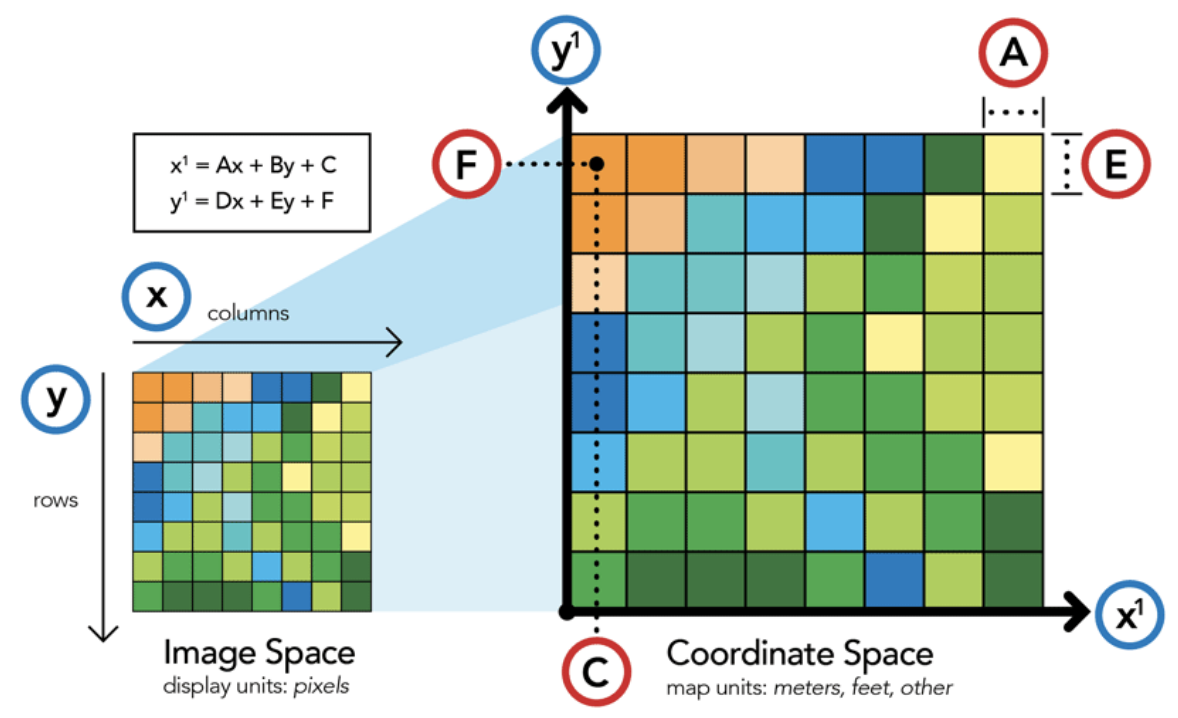
\includegraphics[width=0.75\textwidth]{./image/georref}
	\end{figure}
	\flushright{\tiny{\url{https://www.esri.com/about/newsroom/arcuser/understanding-raster-georeferencing/}}}
\end{frame}

\begin{frame}
	\frametitle{Georreferenciamento de imagens}
	Transformação geométrica de uma imagem através da relação entre as coordenadas da imagem e as coordenadas de um mapa.
	
	\begin{figure}[h]
		\centering
		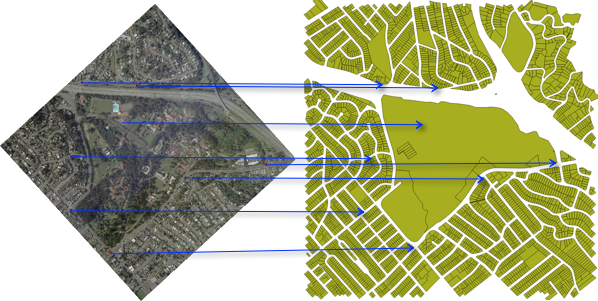
\includegraphics[width=0.85\textwidth]{./image/georref2}
	\end{figure}
	\flushright{\tiny{\url{http://djjr-courses.wikidot.com/soc128:georeferencing-an-image}}}
\end{frame}

\begin{frame}
	\frametitle{Georreferenciamento de imagens}
	Necessário o uso de \textbf{ortofotos}, i.e., uma fotografia aérea livre de distorções.
	
	\begin{figure}[h]
		\centering
		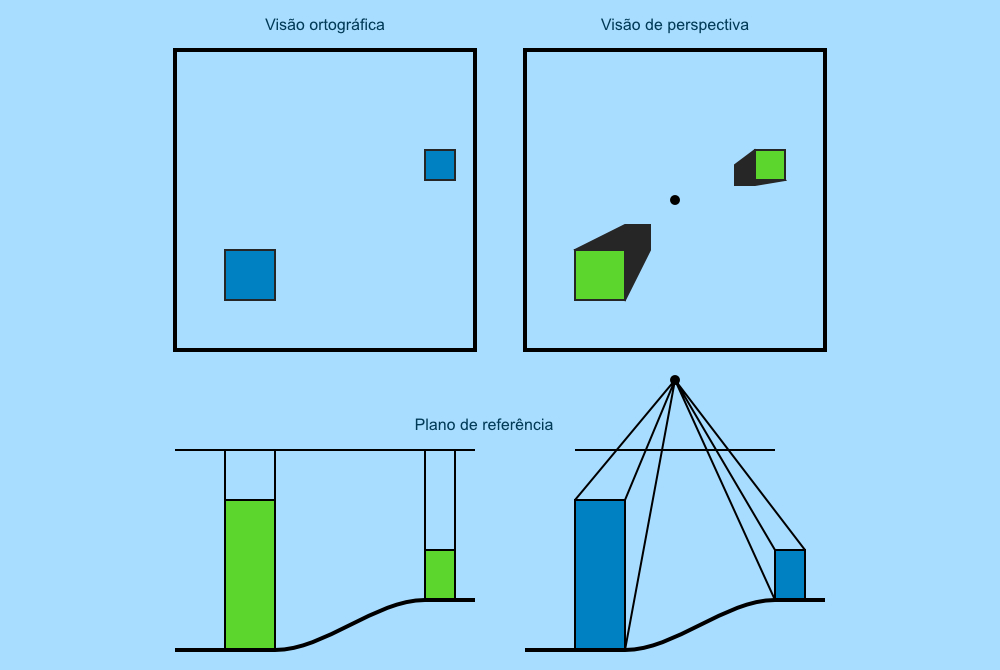
\includegraphics[width=0.65\textwidth]{./image/orto}
	\end{figure}
	\flushright{\tiny{\url{https://www.geosensori.com.br/2019/06/10/o-que-e-ortofoto/}}}
\end{frame}

\begin{frame}
	\frametitle{Georreferenciamento de imagens}
	Ortoimagem frente a uma imagem aérea:
	
	\begin{figure}[h]
		\centering
		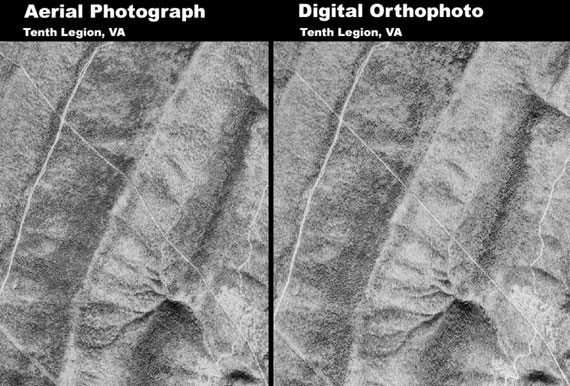
\includegraphics[width=0.7\textwidth]{./image/orto-vs-aer}
	\end{figure}
	\flushright{\tiny{\url{https://www.usgs.gov/media/images/aerial-photograph-vs-orthoimage}}}
\end{frame}

\begin{frame}
	\frametitle{Georreferenciamento de imagens}
	\begin{figure}[H]
		\centering
		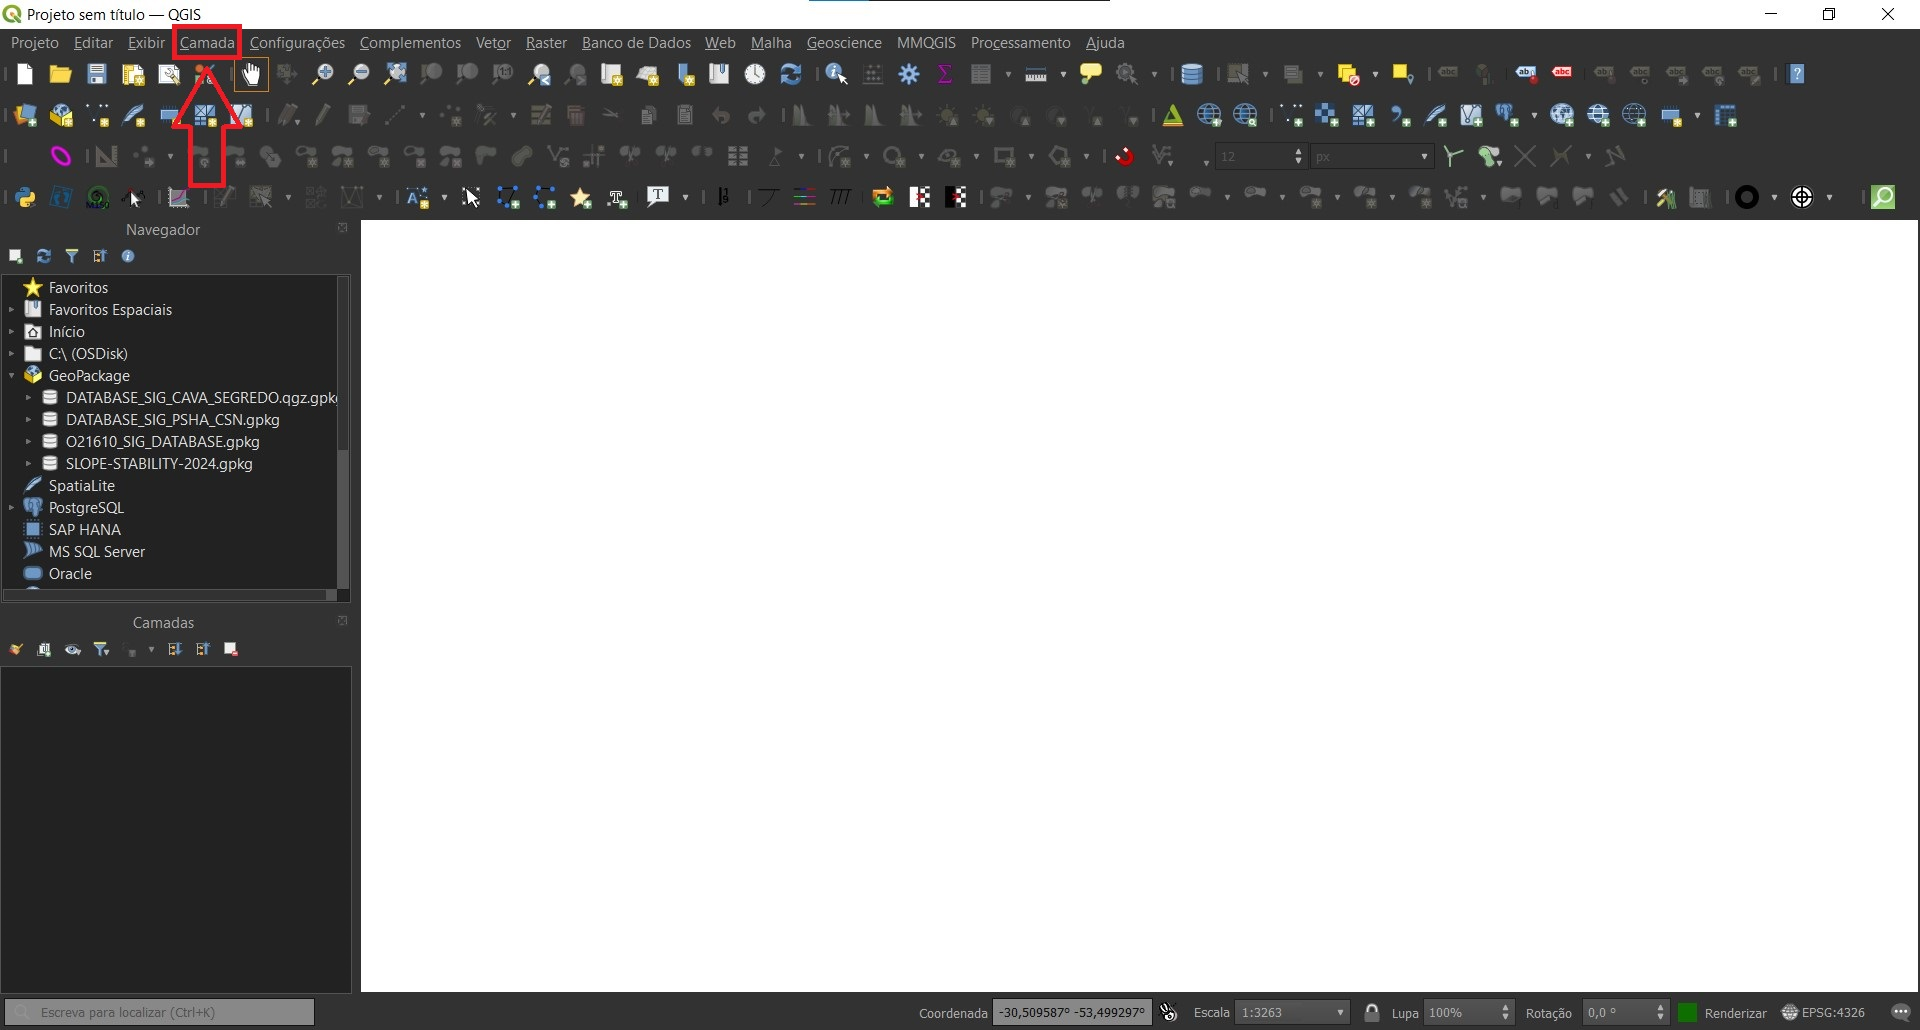
\includegraphics[width=\textwidth]{./image/georref_1}
	\end{figure}
\end{frame}

\begin{frame}
	\frametitle{Georreferenciamento de imagens}
	\begin{figure}[H]
		\centering
		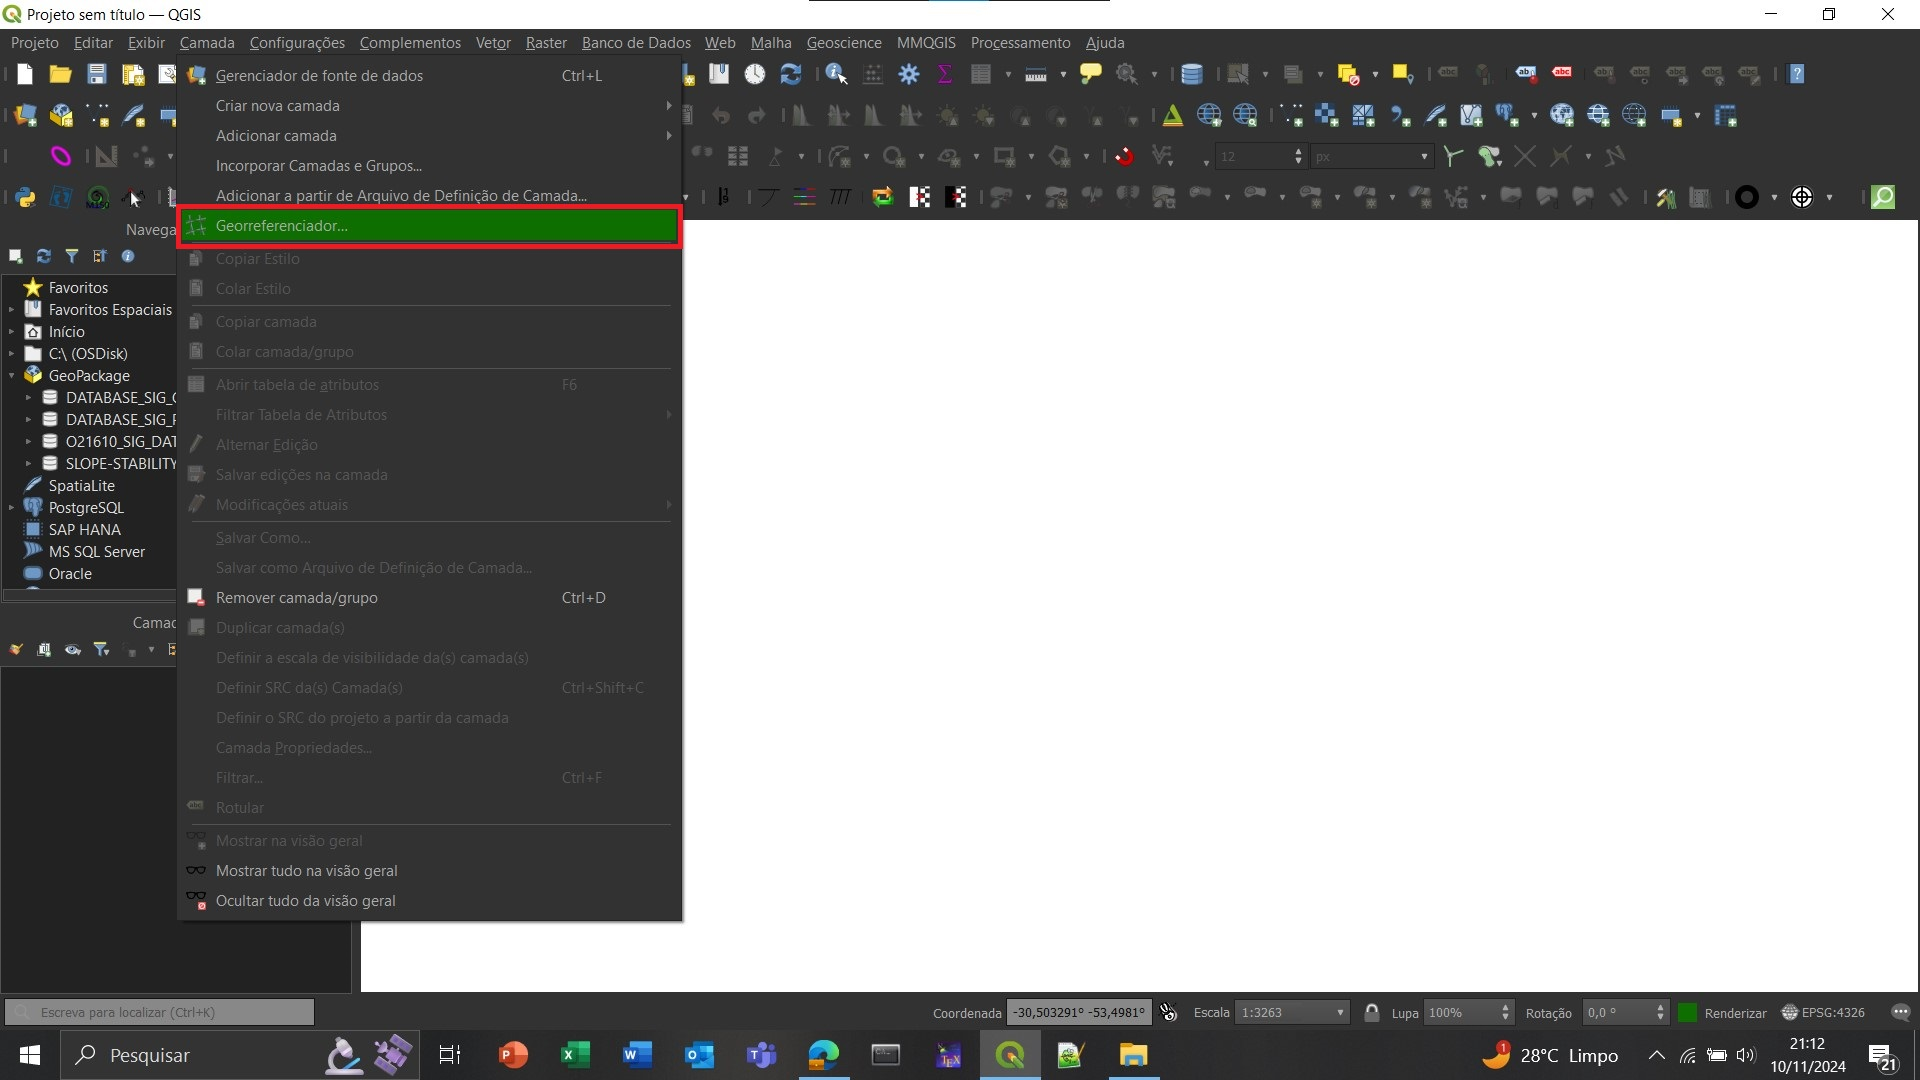
\includegraphics[width=\textwidth]{./image/georref_2}
	\end{figure}
\end{frame}

\begin{frame}
	\frametitle{Georreferenciamento de imagens}
	\begin{figure}[H]
		\centering
		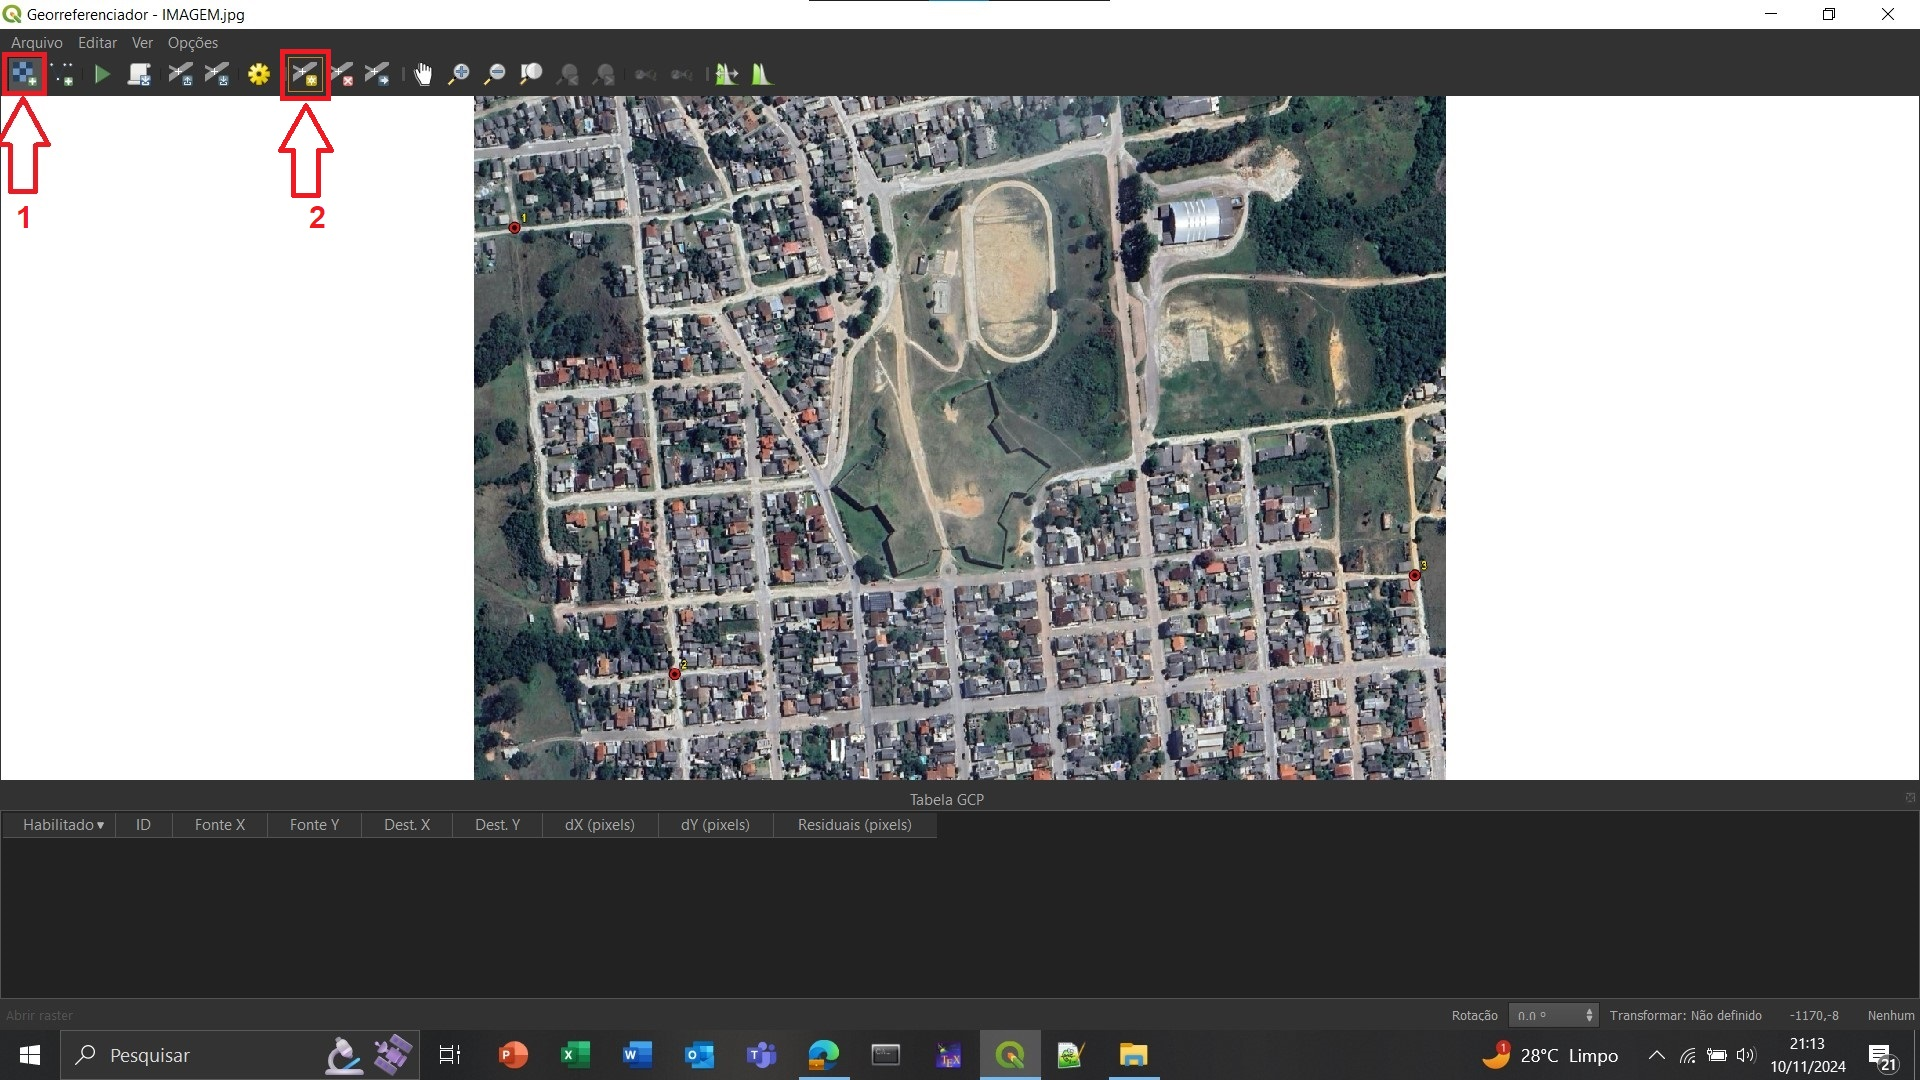
\includegraphics[width=\textwidth]{./image/georref_3}
	\end{figure}
\end{frame}

\begin{frame}
	\frametitle{Georreferenciamento de imagens}
	\begin{figure}[H]
		\centering
		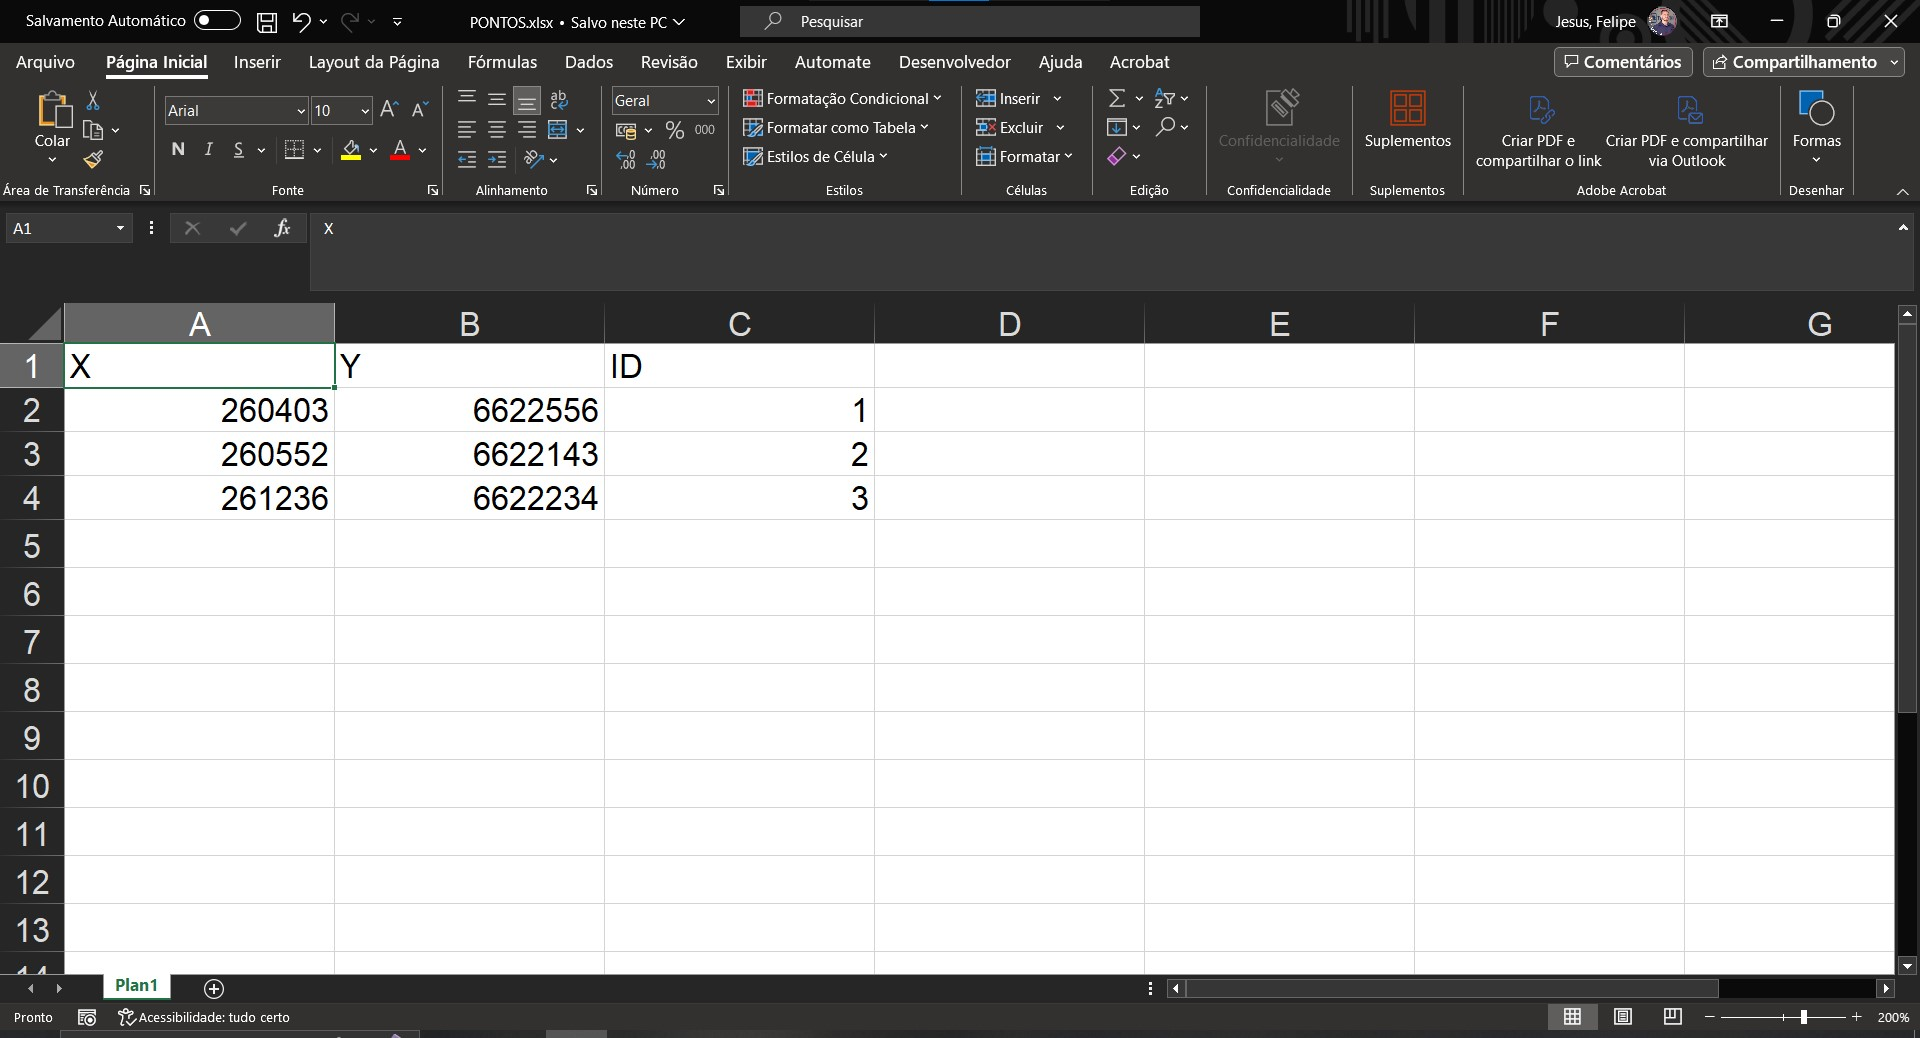
\includegraphics[width=\textwidth]{./image/georref_4}
	\end{figure}
\end{frame}

\begin{frame}
	\frametitle{Georreferenciamento de imagens}
	\begin{figure}[H]
		\centering
		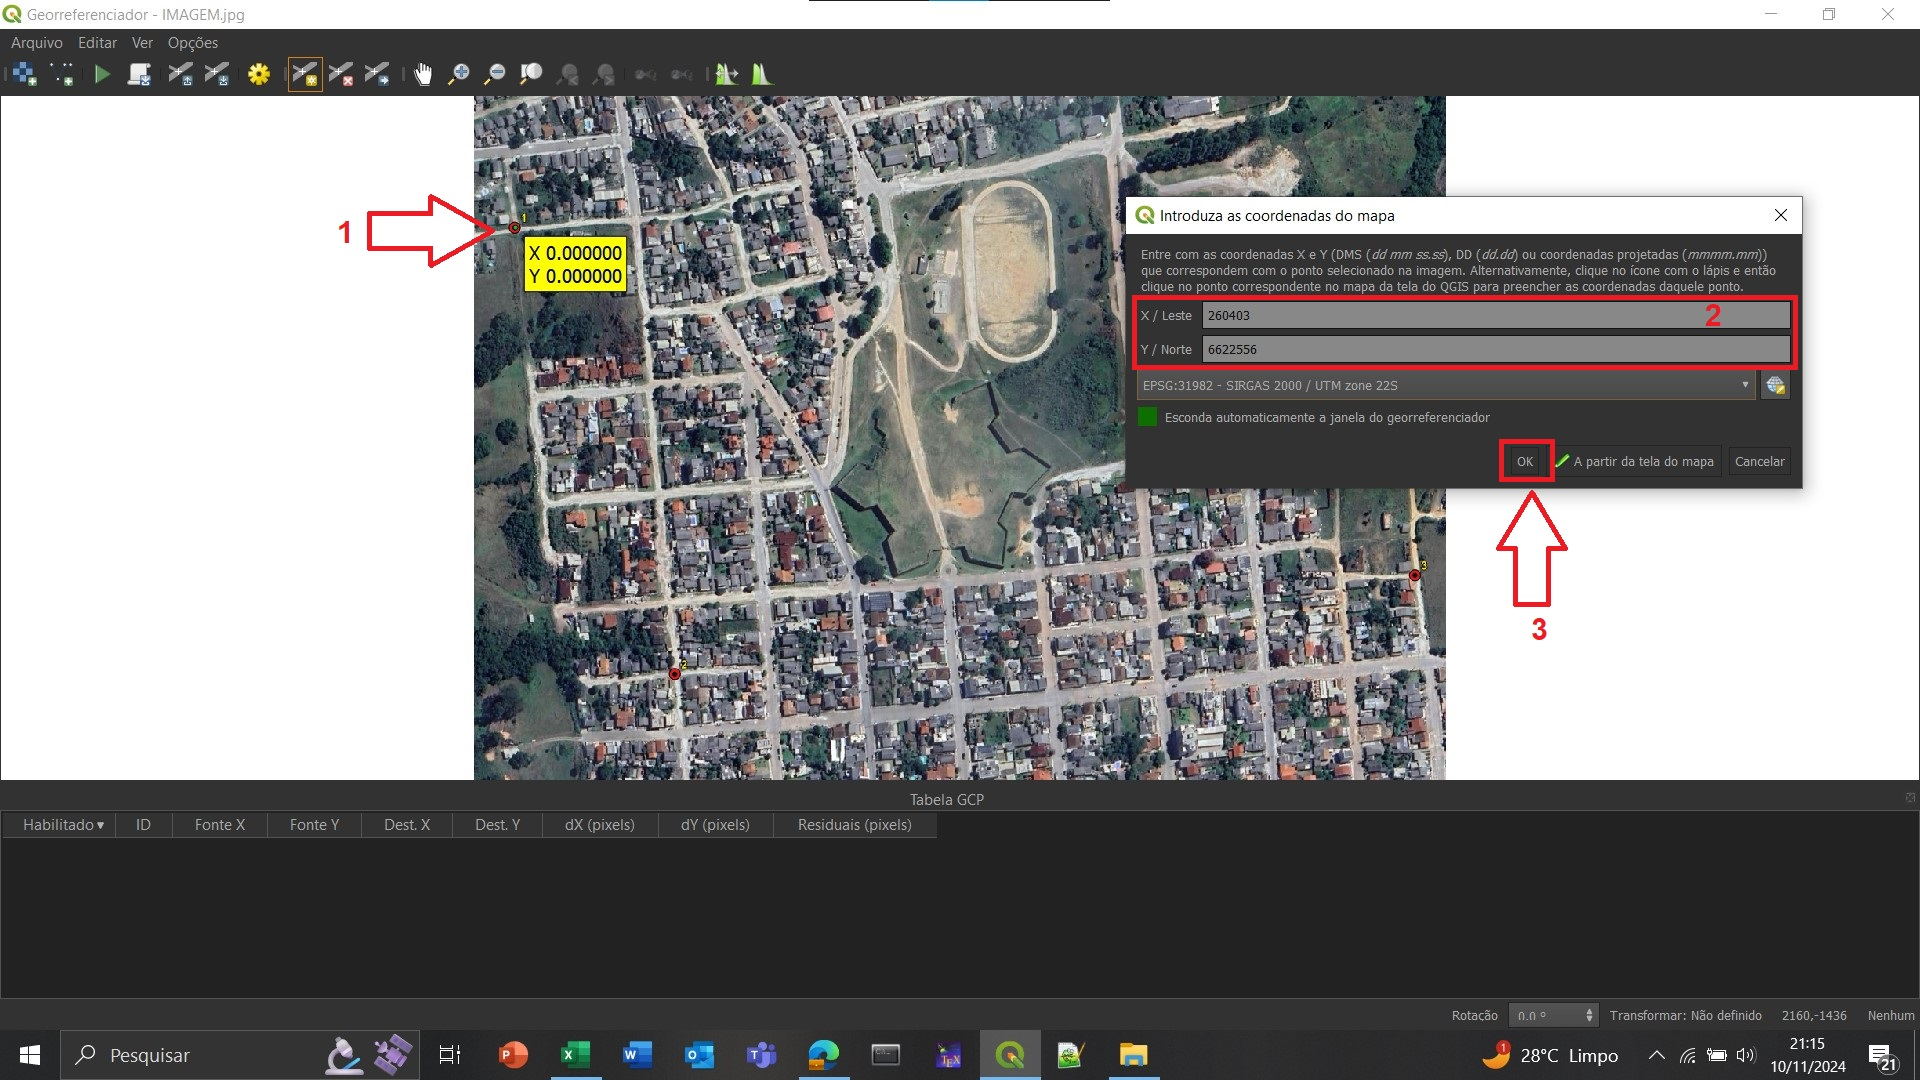
\includegraphics[width=\textwidth]{./image/georref_5}
	\end{figure}
\end{frame}

\begin{frame}
	\frametitle{Georreferenciamento de imagens}
	\begin{figure}[H]
		\centering
		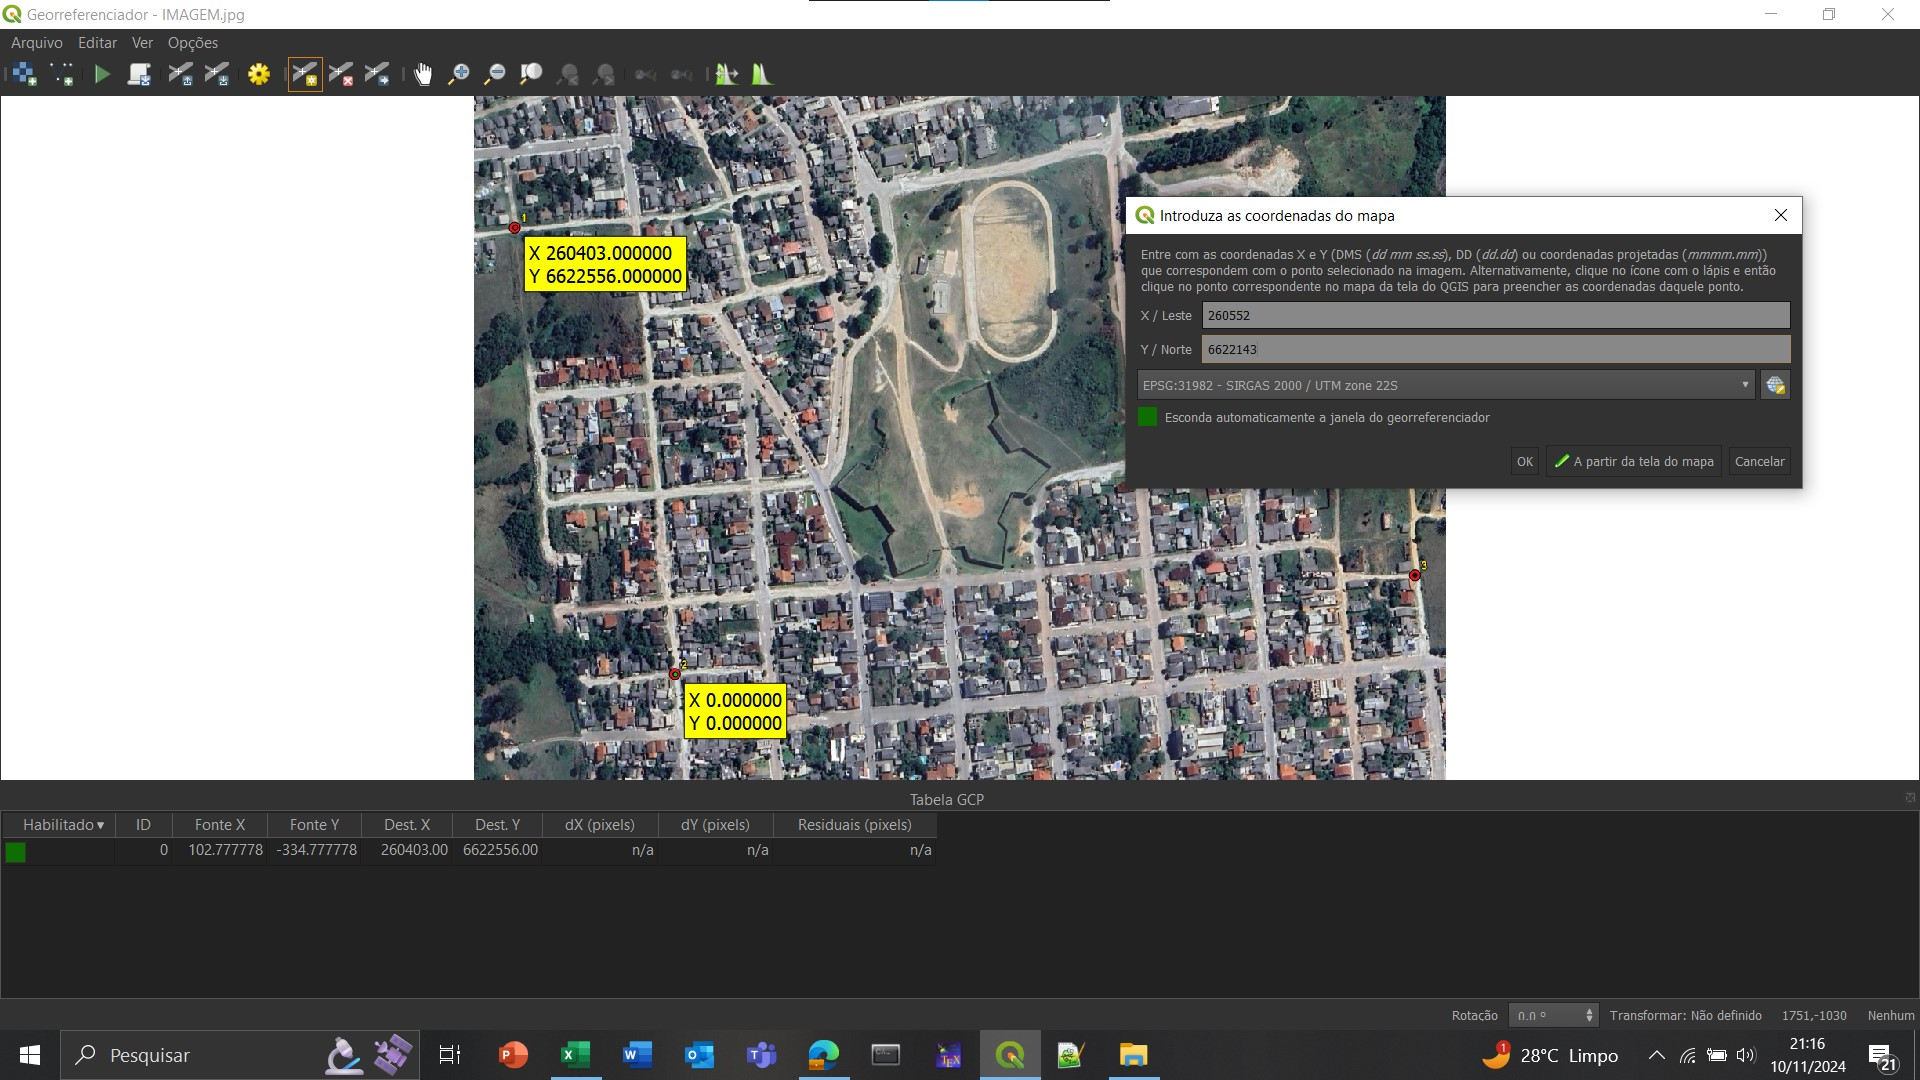
\includegraphics[width=\textwidth]{./image/georref_6}
	\end{figure}
\end{frame}

\begin{frame}
	\frametitle{Georreferenciamento de imagens}
	\begin{figure}[H]
		\centering
		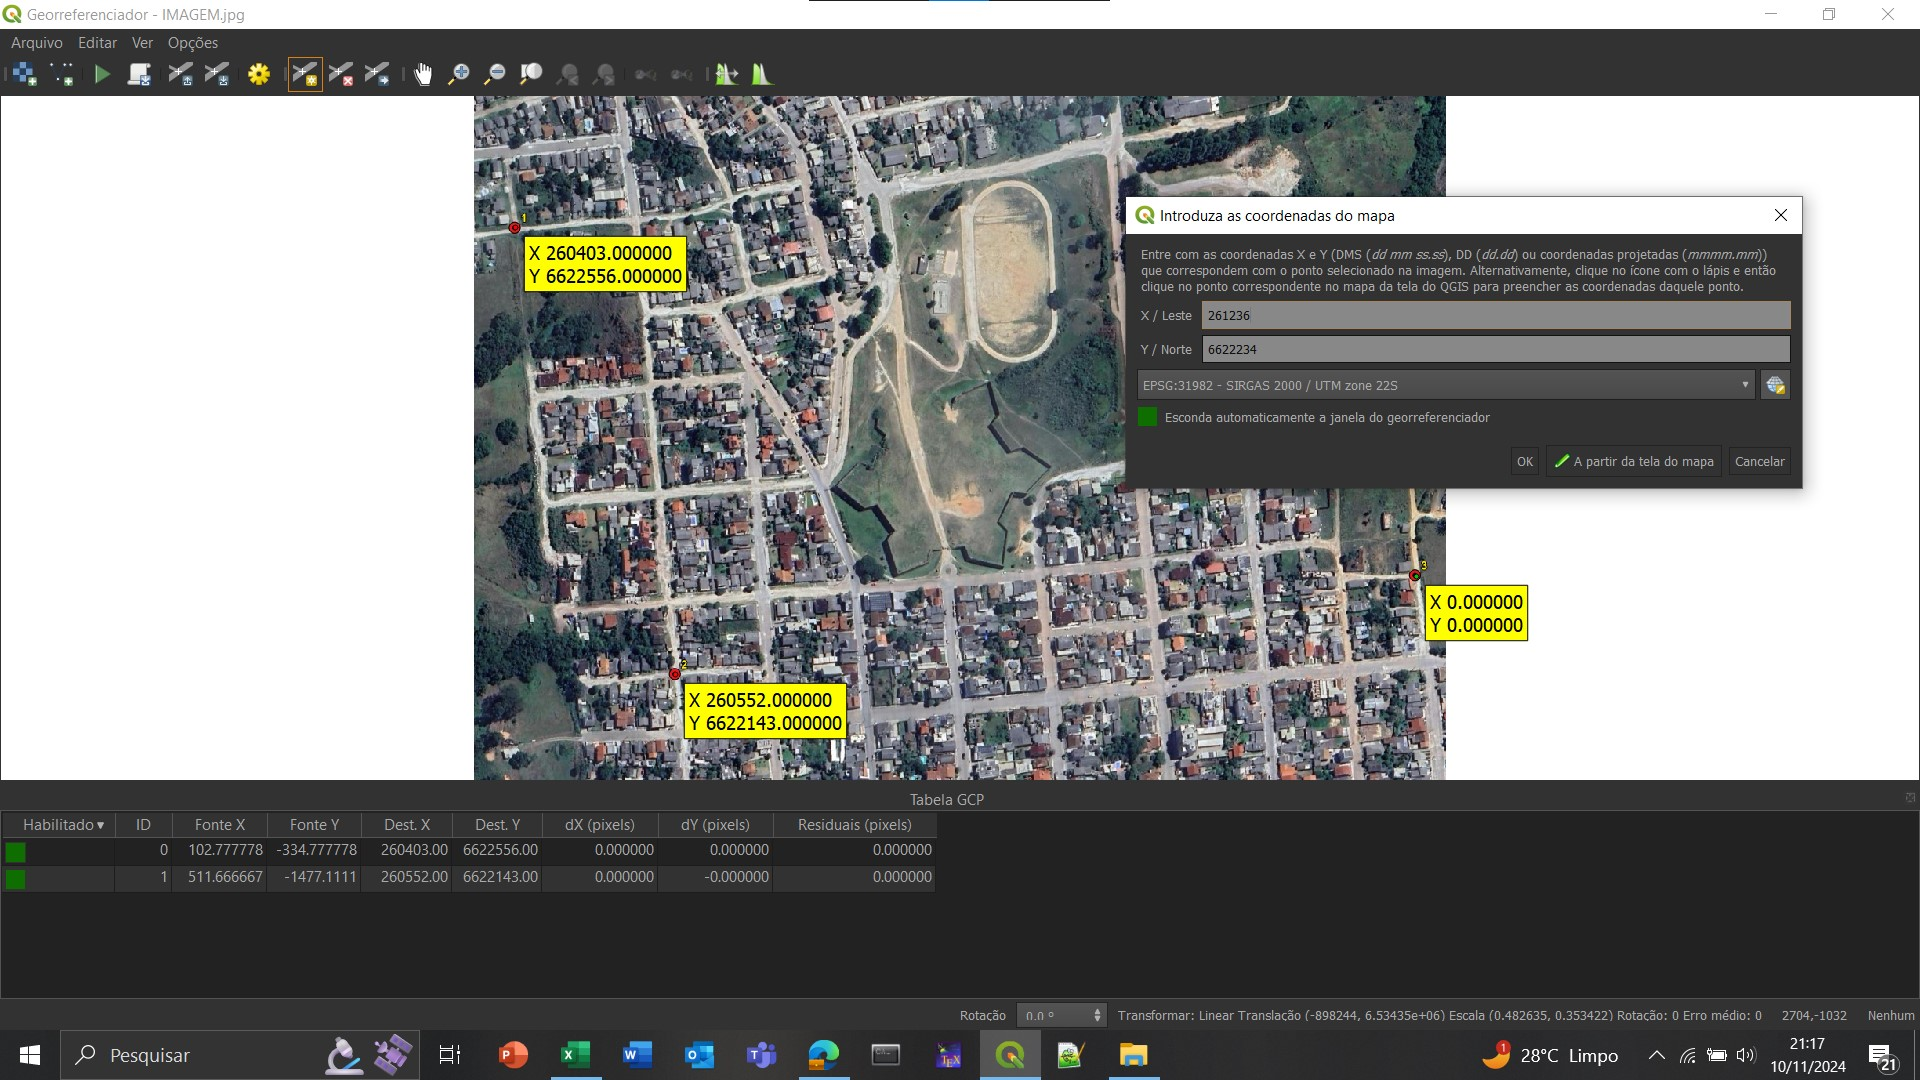
\includegraphics[width=\textwidth]{./image/georref_7}
	\end{figure}
\end{frame}

\begin{frame}
	\frametitle{Georreferenciamento de imagens}
	\begin{figure}[H]
		\centering
		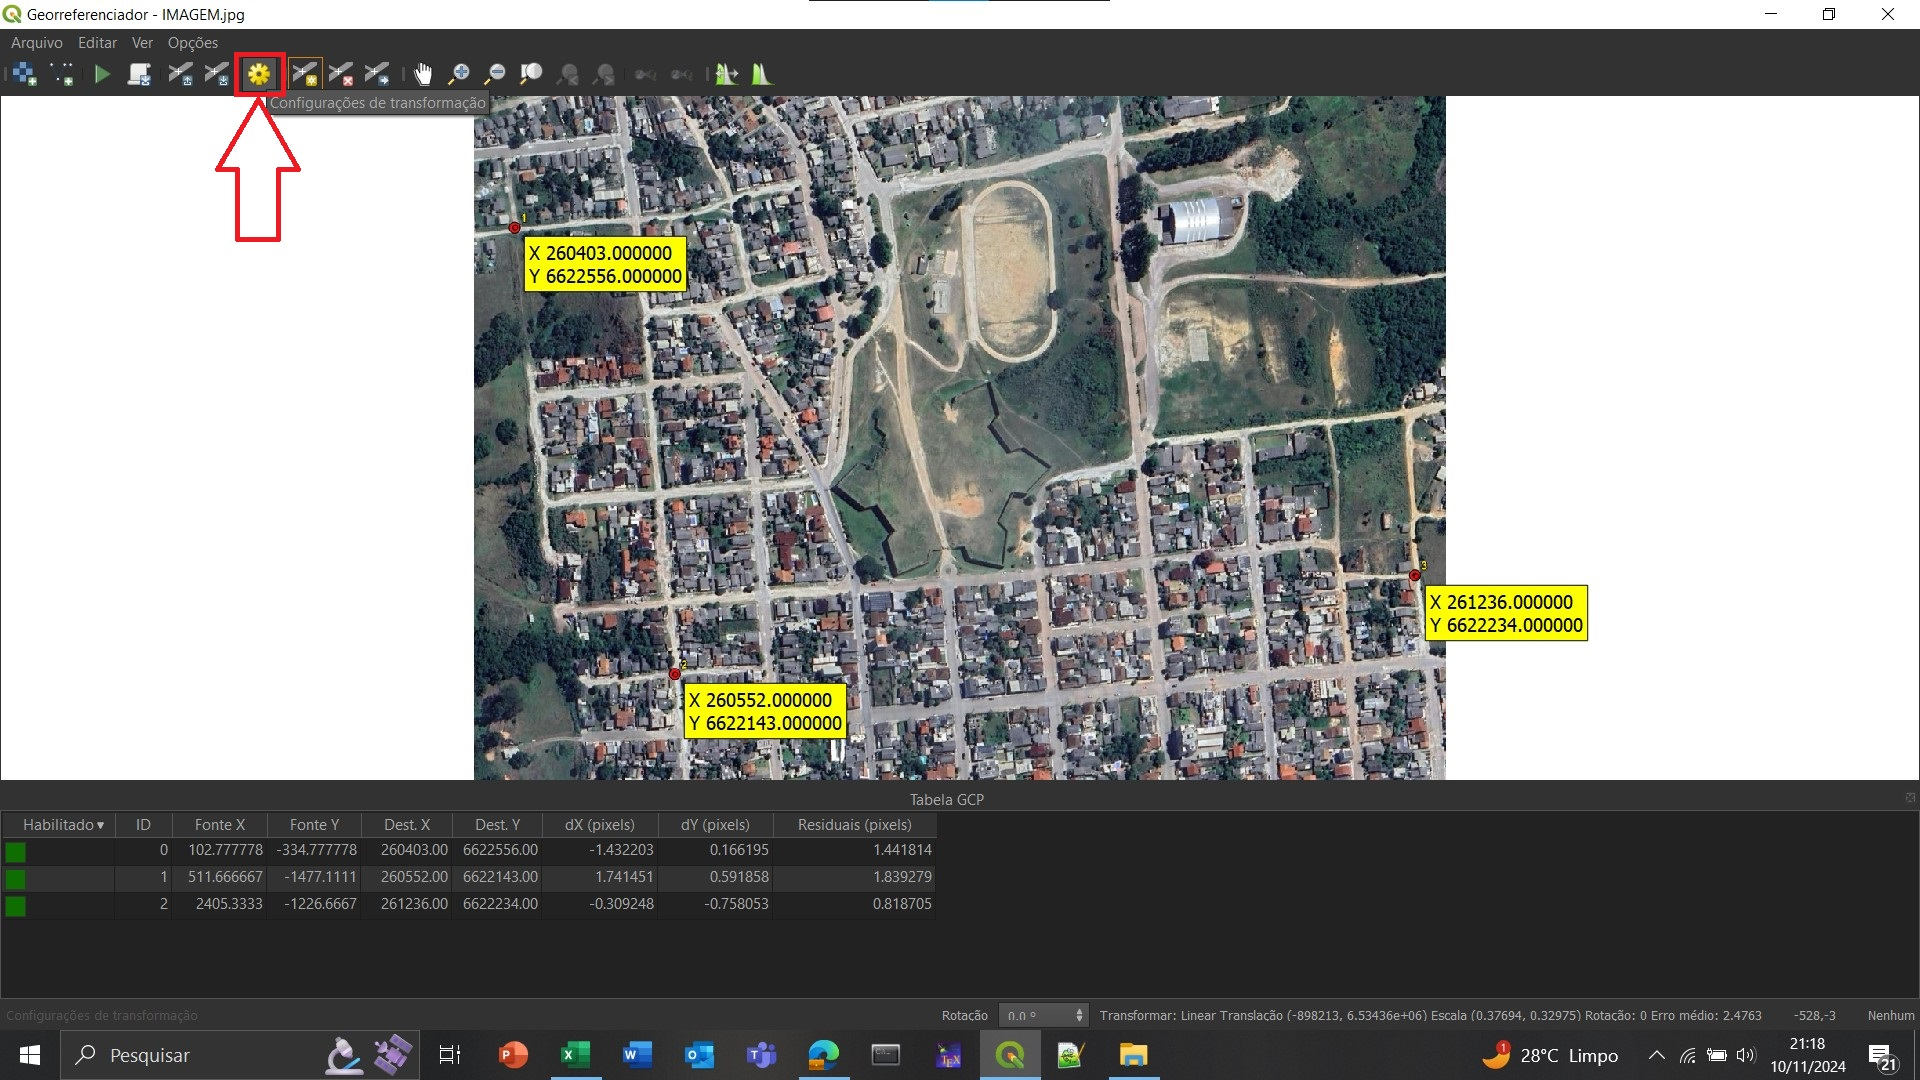
\includegraphics[width=\textwidth]{./image/georref_8}
	\end{figure}
\end{frame}

\begin{frame}
	\frametitle{Georreferenciamento de imagens}
	\begin{figure}[H]
		\centering
		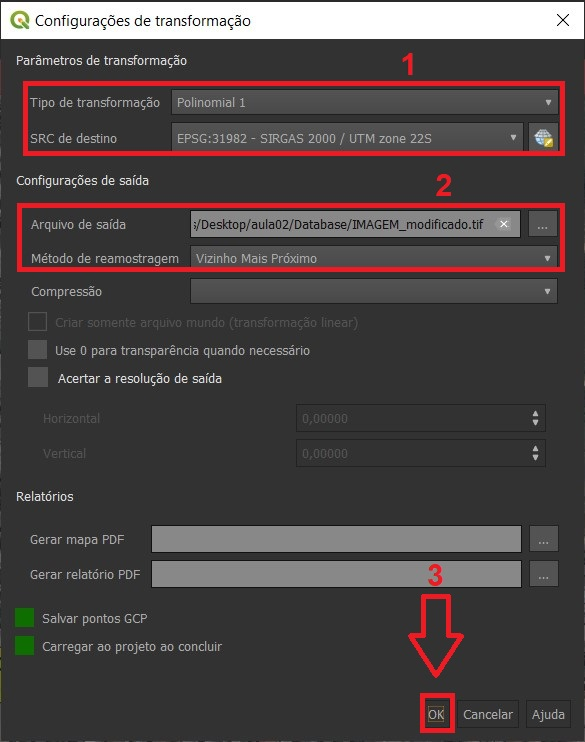
\includegraphics[width=0.5\textwidth]{./image/georref_9}
	\end{figure}
\end{frame}

\begin{frame}
	\frametitle{Georreferenciamento de imagens}
	\begin{figure}[H]
		\centering
		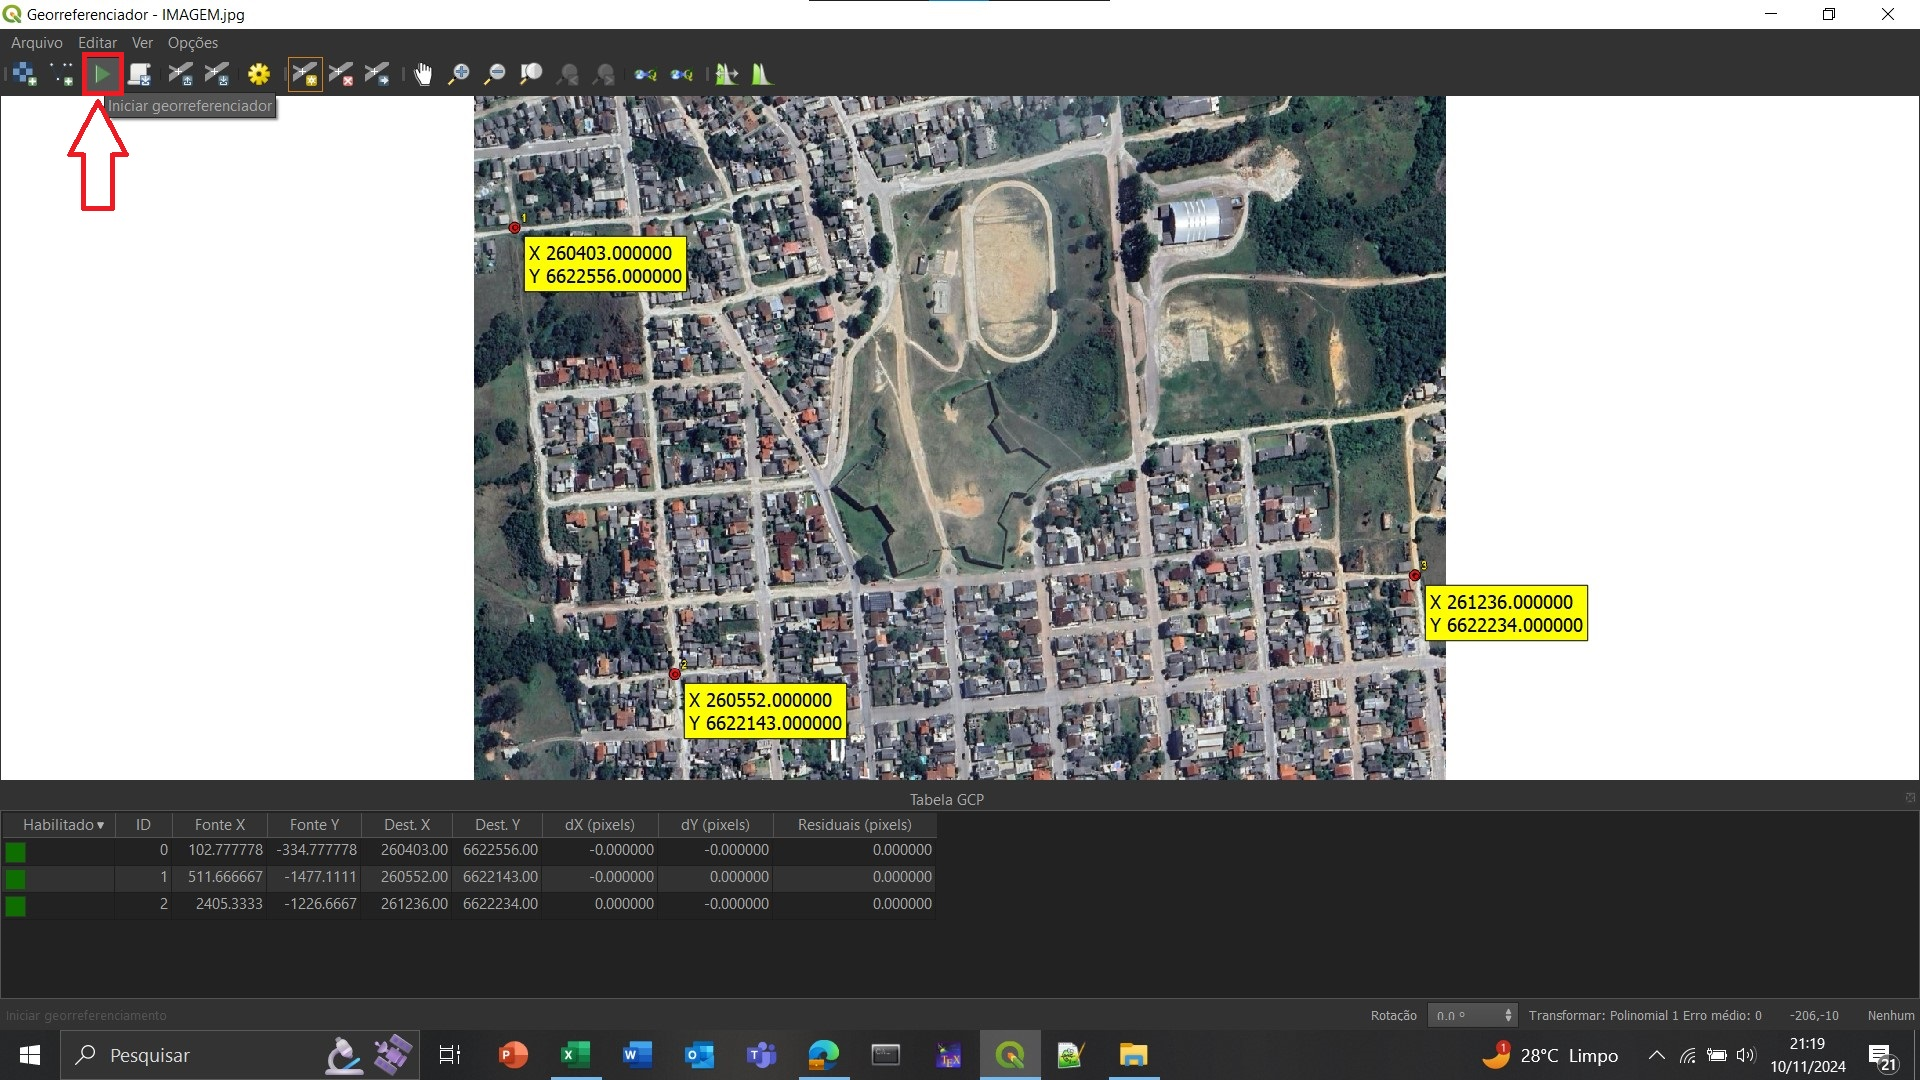
\includegraphics[width=\textwidth]{./image/georref_10}
	\end{figure}
\end{frame}

\begin{frame}
	\frametitle{Georreferenciamento de imagens}
	\begin{figure}[H]
		\centering
		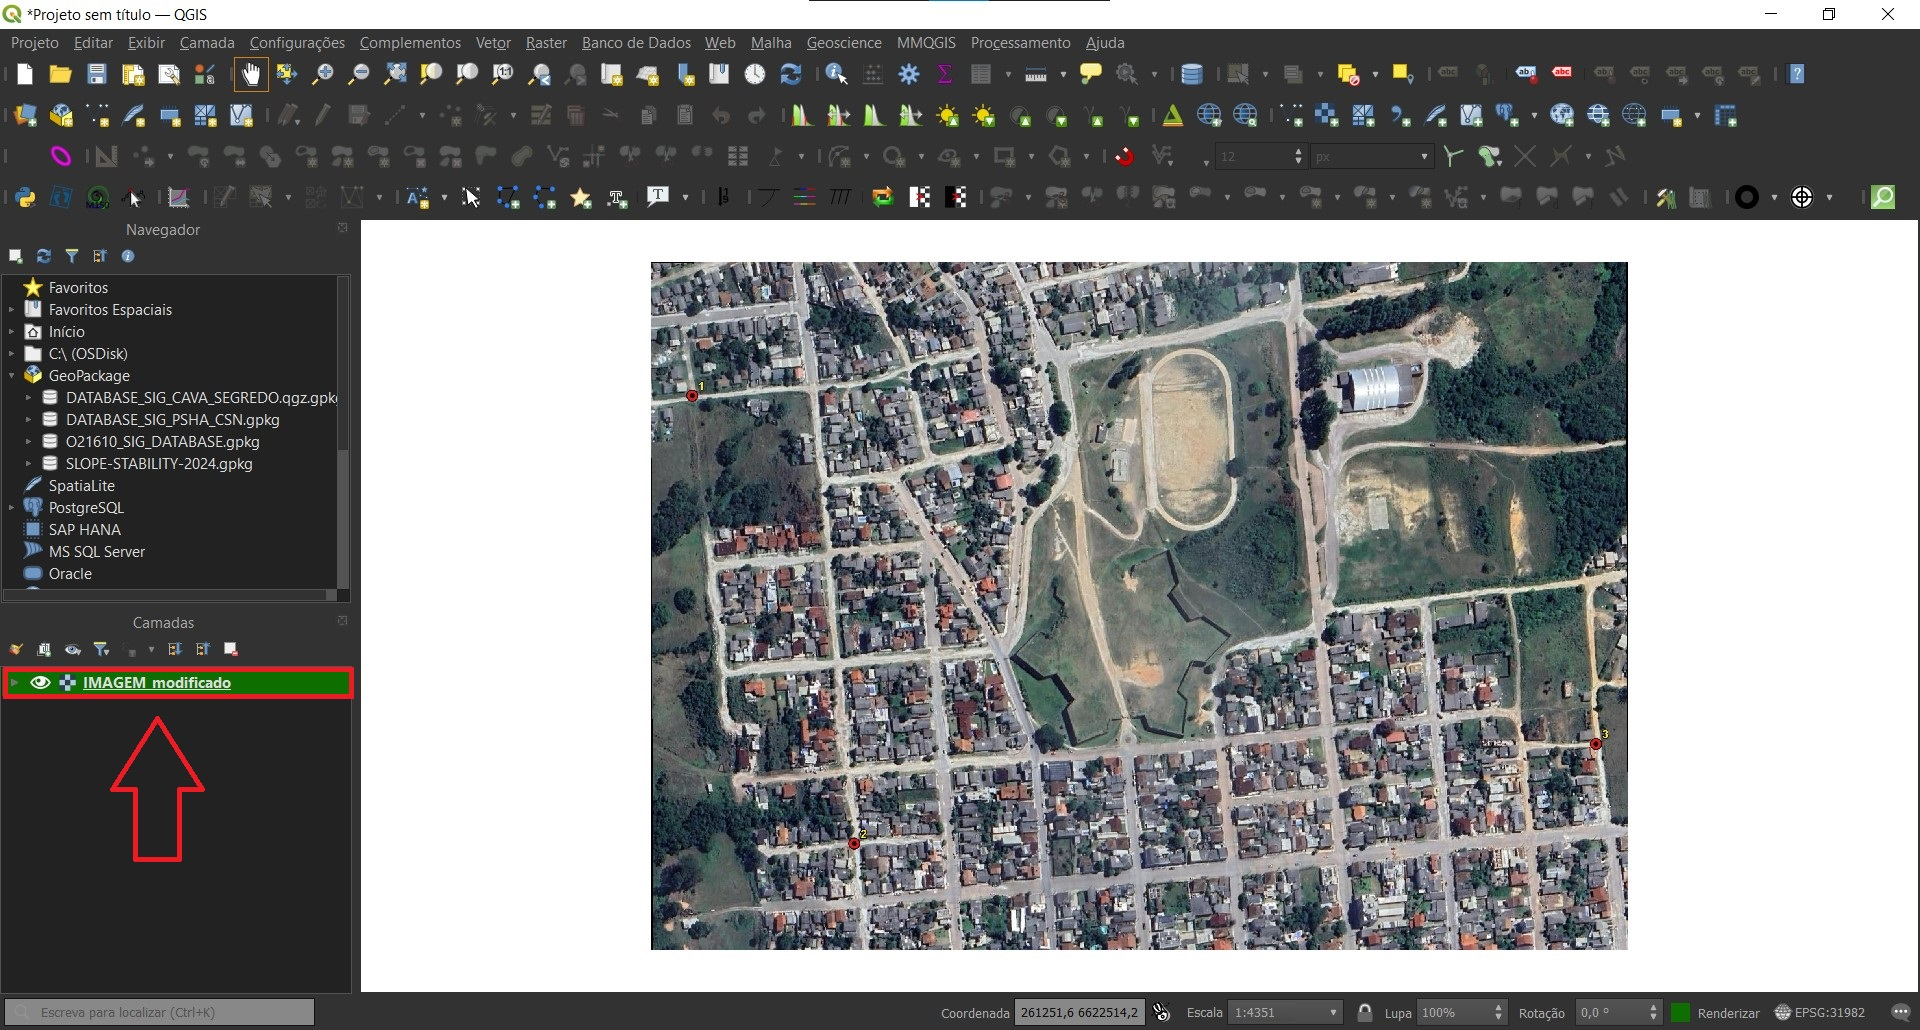
\includegraphics[width=\textwidth]{./image/georref_11}
	\end{figure}
\end{frame}

\begin{frame}
	\frametitle{Georreferenciamento de imagens}
	\begin{figure}[H]
		\centering
		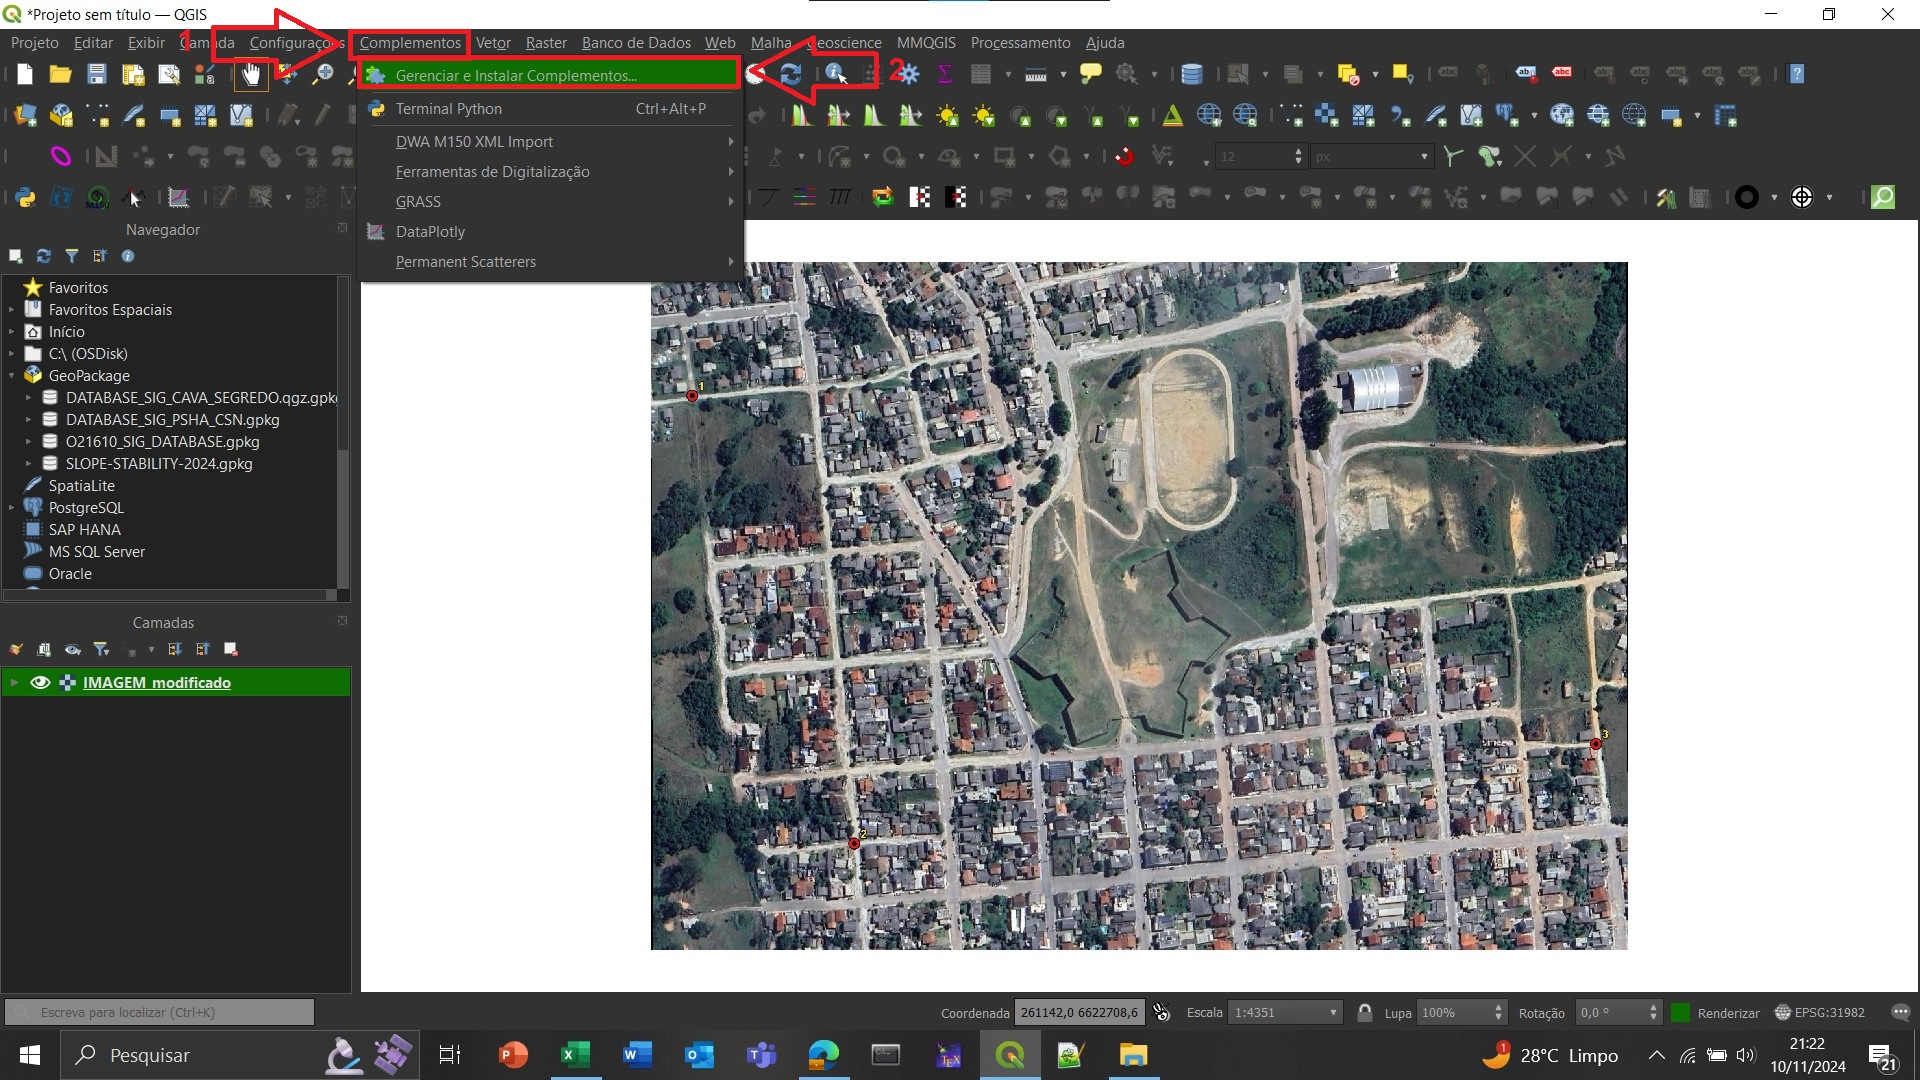
\includegraphics[width=\textwidth]{./image/georref_12}
	\end{figure}
\end{frame}

\begin{frame}
	\frametitle{Georreferenciamento de imagens}
	\begin{figure}[H]
		\centering
		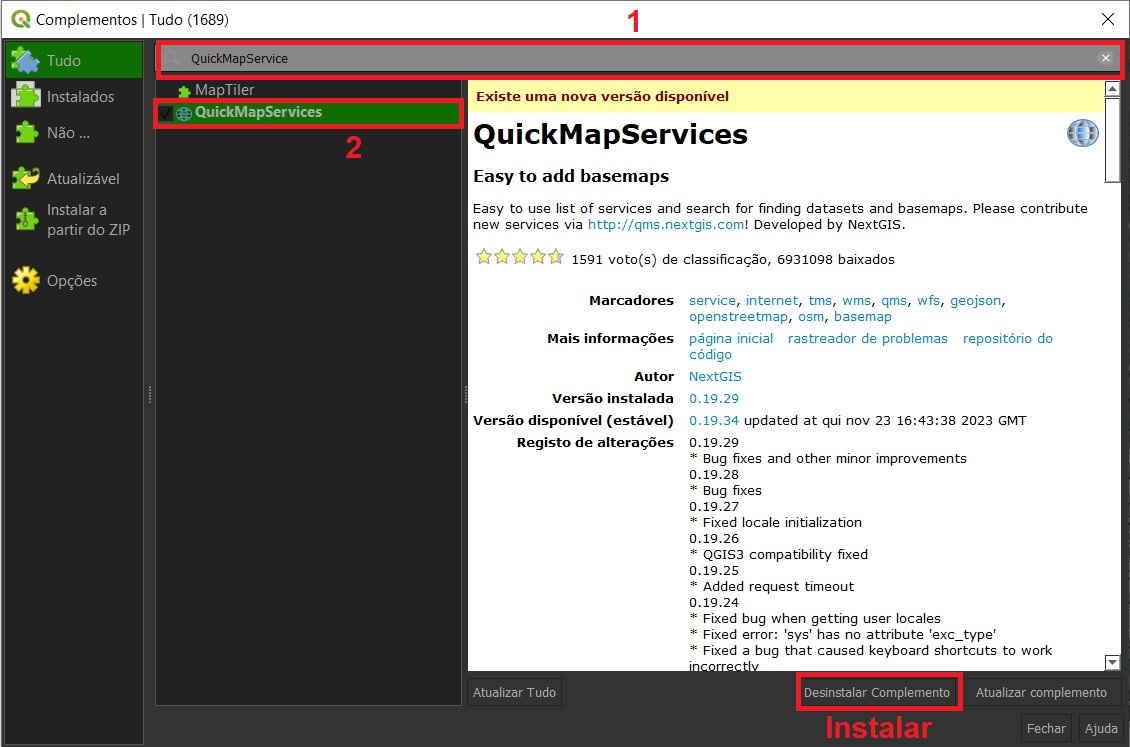
\includegraphics[width=\textwidth]{./image/georref_13}
	\end{figure}
\end{frame}

\begin{frame}
	\frametitle{Georreferenciamento de imagens}
	\begin{figure}[H]
		\centering
		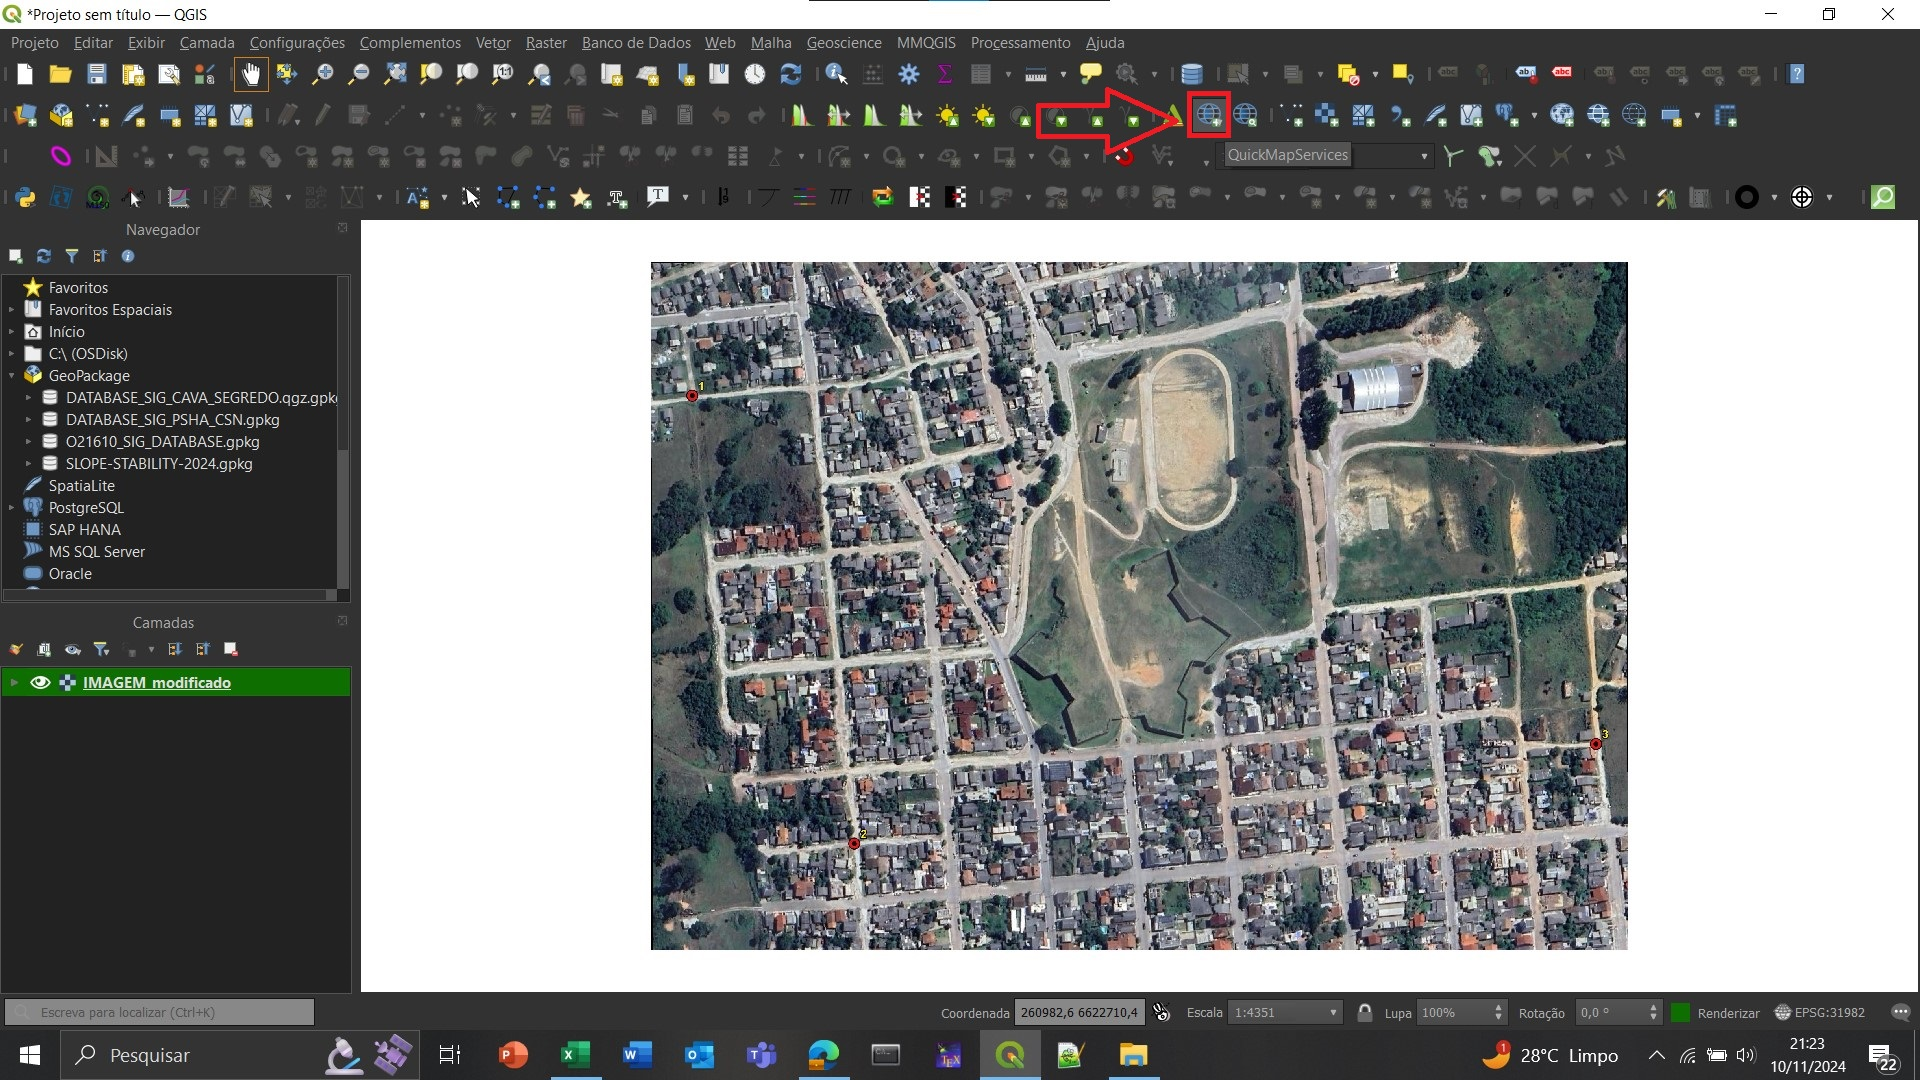
\includegraphics[width=\textwidth]{./image/georref_14}
	\end{figure}
\end{frame}

\begin{frame}
	\frametitle{Georreferenciamento de imagens}
	\begin{figure}[H]
		\centering
		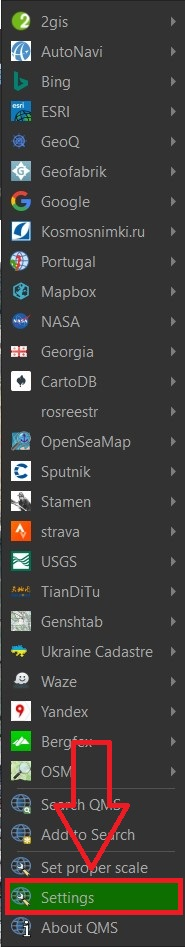
\includegraphics[width=0.13\textwidth]{./image/georref_15}
	\end{figure}
\end{frame}

\begin{frame}
	\frametitle{Georreferenciamento de imagens}
	\begin{figure}[H]
		\centering
		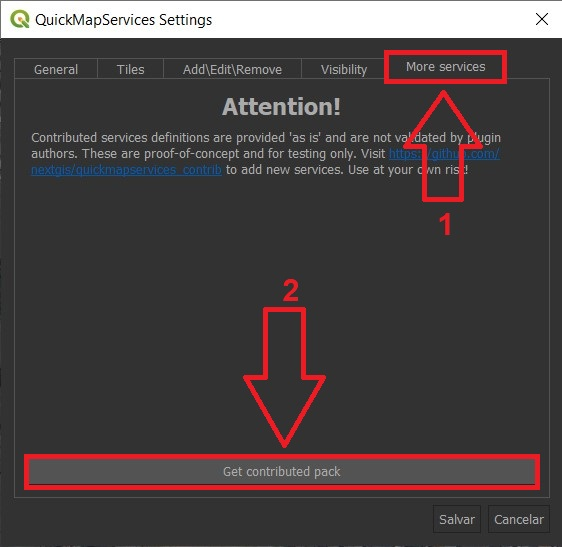
\includegraphics[width=0.65\textwidth]{./image/georref_16}
	\end{figure}
\end{frame}

\begin{frame}
	\frametitle{Georreferenciamento de imagens}
	\begin{figure}[H]
		\centering
		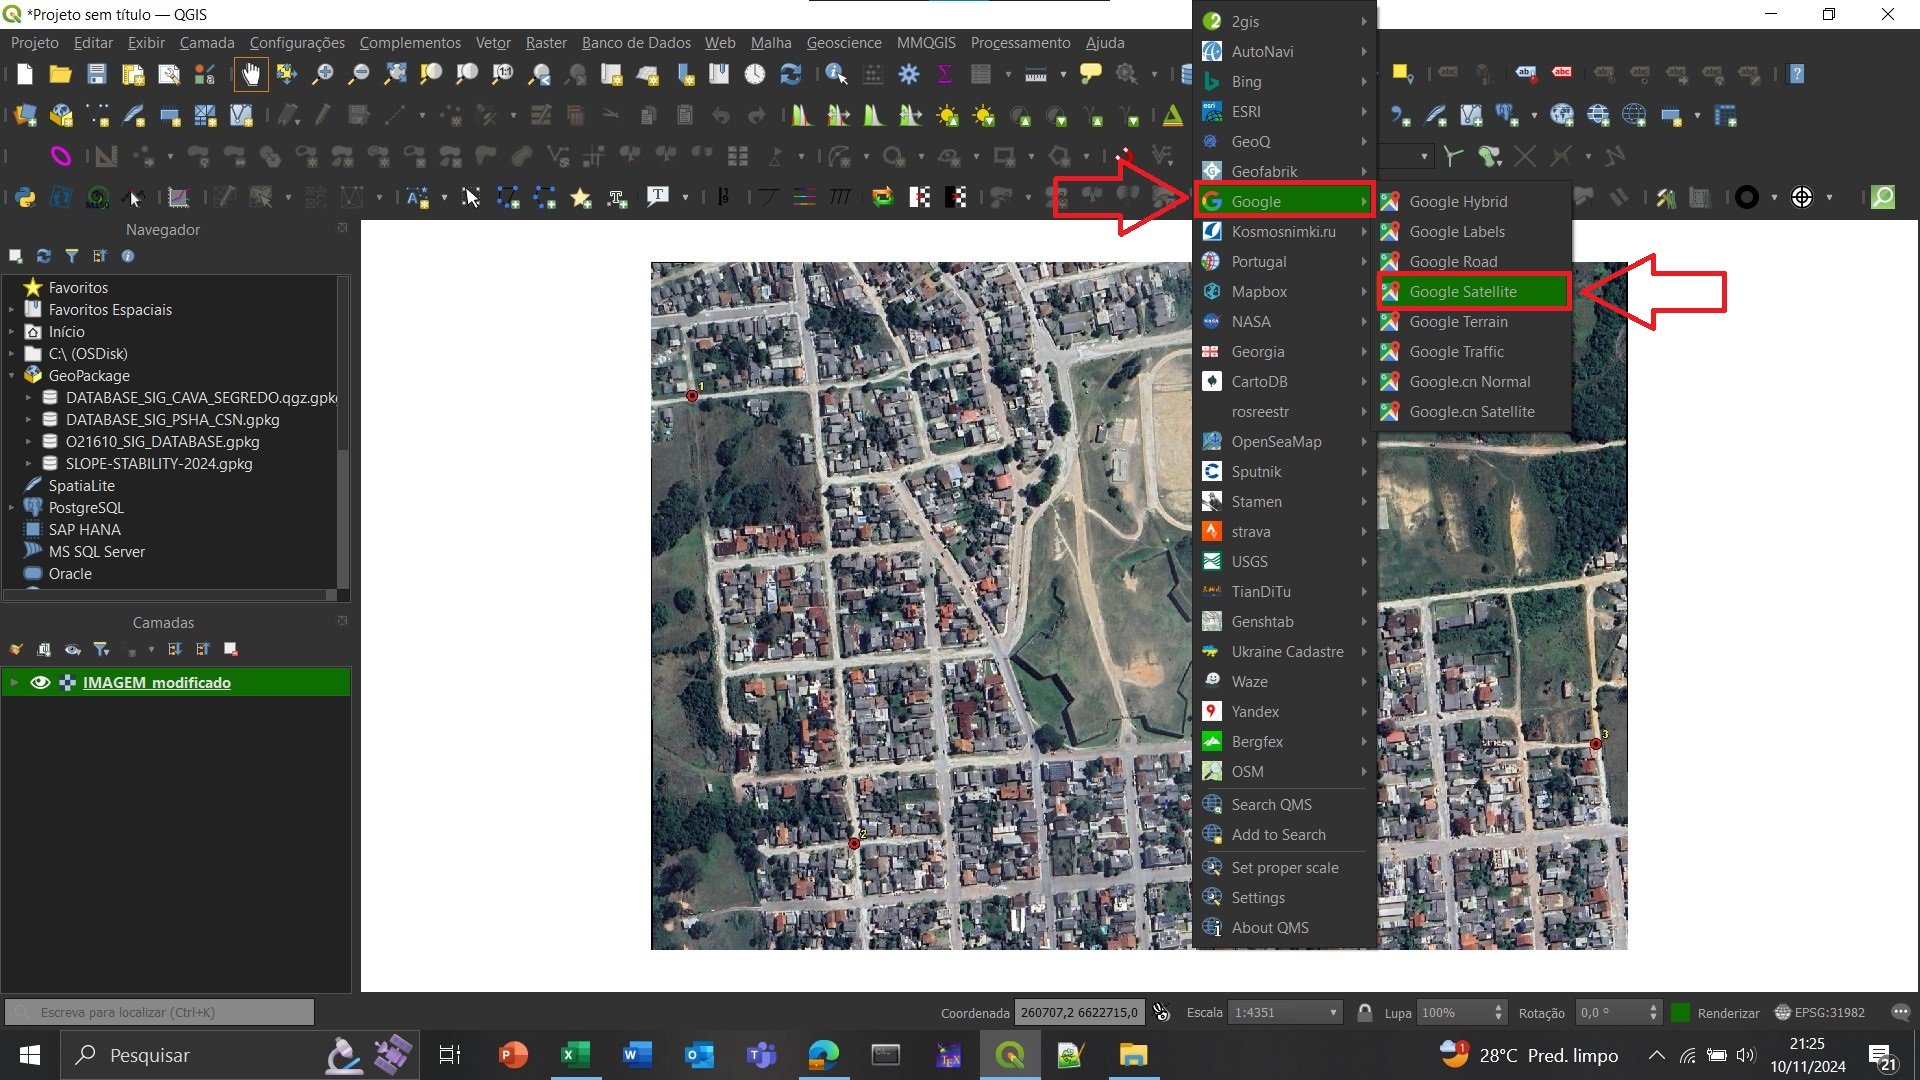
\includegraphics[width=\textwidth]{./image/georref_17}
	\end{figure}
\end{frame}

\begin{frame}
	\frametitle{Georreferenciamento de imagens}
	\begin{figure}[H]
		\centering
		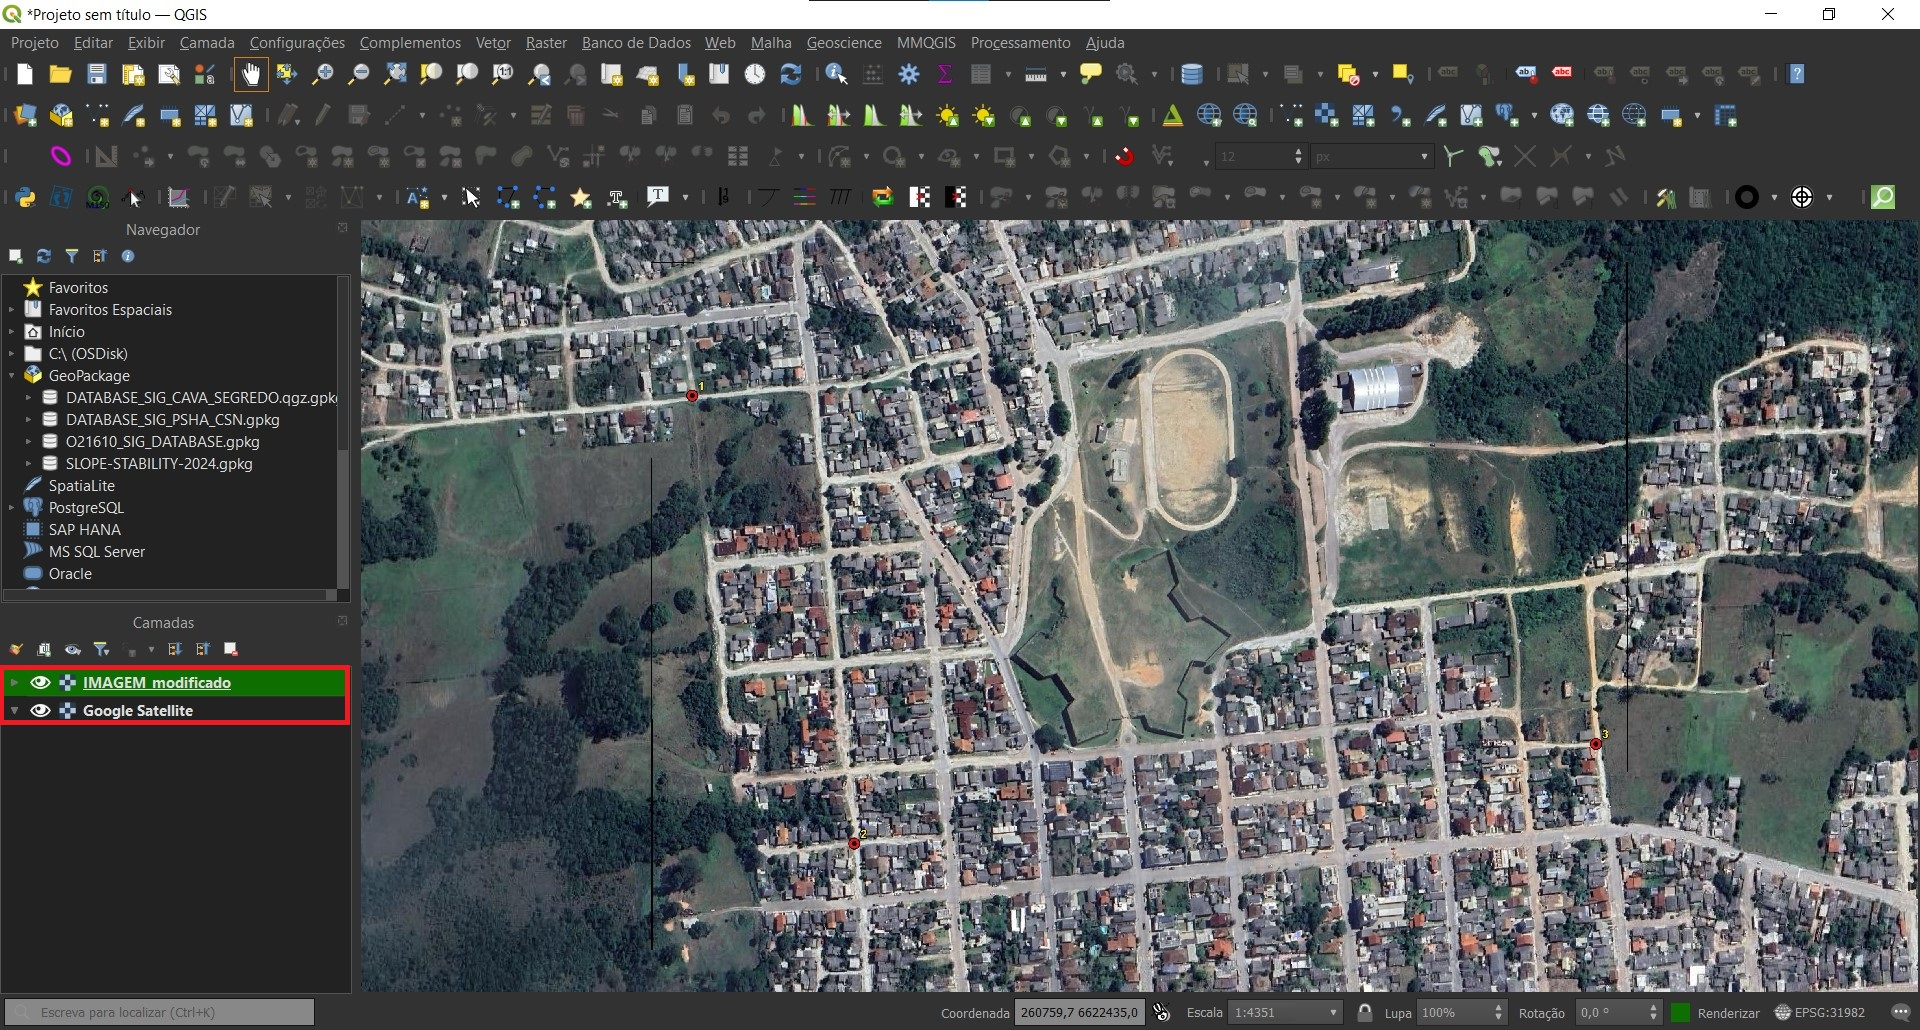
\includegraphics[width=\textwidth]{./image/georref_18}
	\end{figure}
\end{frame}

\begin{frame}
	\frametitle{Georreferenciamento de imagens}
	\begin{figure}[H]
		\centering
		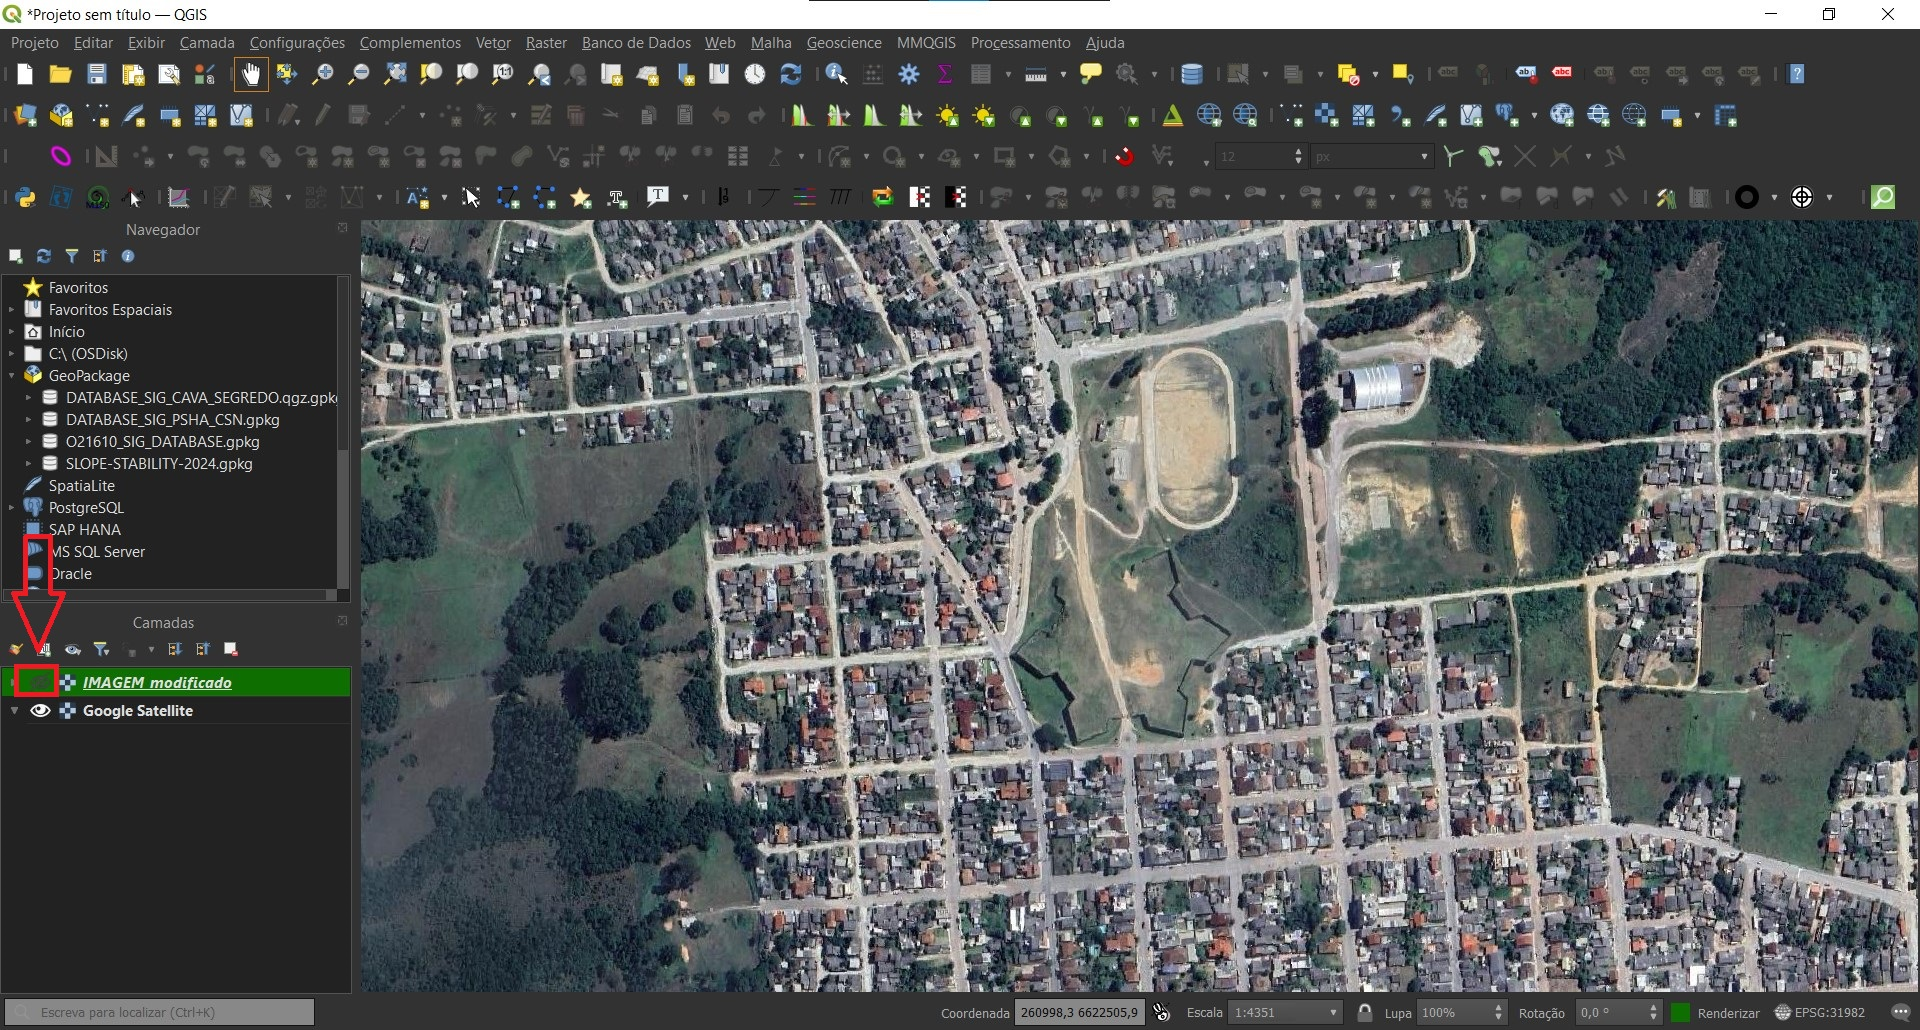
\includegraphics[width=\textwidth]{./image/georref_19}
	\end{figure}
\end{frame}

\begin{frame}
	\frametitle{Georreferenciamento de imagens}
	\begin{figure}[H]
		\centering
		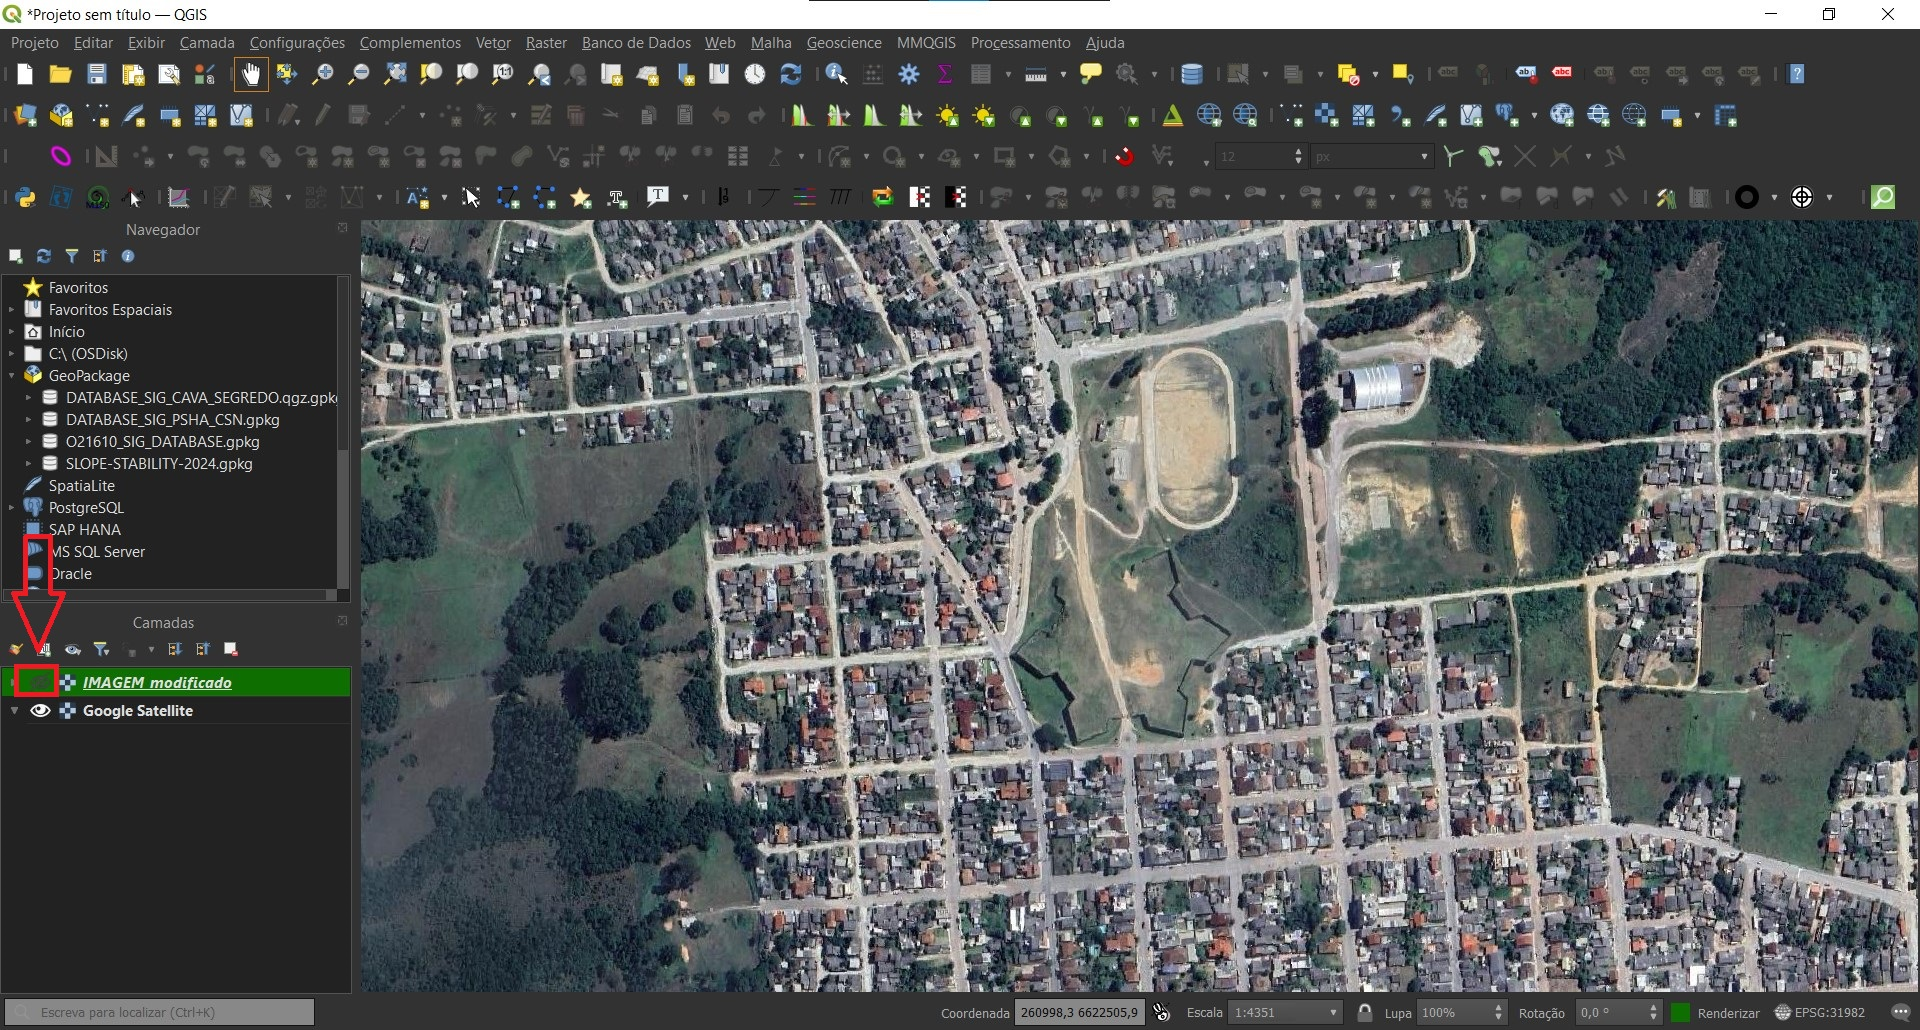
\includegraphics[width=\textwidth]{./image/georref_19}
	\end{figure}
\end{frame}

\begin{frame}
	\frametitle{Levantamento de imagem aérea}
	\begin{figure}[H]
		\centering
		\vspace{1cm}
		
\includegraphics[width=0.85\textwidth]{./image/topgun}
	\end{figure}
\end{frame}

\begin{frame}
	\frametitle{Levantamento de imagem aérea}
	\begin{figure}[H]
		\centering
		
\includegraphics[width=0.65\textwidth]{./image/infinito}
	\end{figure}
\end{frame}

\end{document}